\documentclass[14pt]{book}
\usepackage{multicol}
\usepackage{amsmath}
\usepackage{amsthm}
\usepackage{graphicx}
\usepackage{color}
\usepackage[utf8]{inputenc}
\usepackage{framed,enumitem} 
\usepackage{pdfpages} 
\usepackage[english]{babel}
%\newenvironment{proof}{\paragraph{Proof:}}{\hfill$\square$}
\usepackage{mathrsfs}
\usepackage{commath}
\usepackage{empheq,mathtools}
\usepackage[backend=biber, style=authortitle]{biblatex}
\addbibresource{/home/ensimag/Documents/notes/fall\_2019/references.bib}
\usepackage{mdframed}
\usepackage{multicol}
\usepackage{enumitem}
%\usepackage{unicode-math}
\usepackage[makeroom]{cancel}
\usepackage{import}
\usepackage{xifthen}
\usepackage{transparent}
\usepackage{amssymb}
\usepackage{tabularx}
\usepackage[bookmarks]{hyperref}
\newcommand{\incfig}[1]{%
    \def\svgwidth{\columnwidth}
    \import{./figures/}{#1.pdf_tex}
}
\pdfsuppresswarningpagegroup=1


\setcounter{tocdepth}{2}
\setcounter{secnumdepth}{2}

\newtheorem{theo}{Theorem}[section] % reset theorem numbering for each chapter
\newtheorem{defn}[theo]{Definition} % definition numbers are dependent on theorem numbers
\newtheorem{exmp}[theo]{Example} % same for example numbers
\newtheorem{cor}[theo]{Corollary} % same for corollary numbers
\newtheorem{prop}[theo]{Proposition} % same 

%make ftheo be framed theorems
\newenvironment{ftheo}
  {\begin{mdframed}\begin{theo}}
  {\end{theo}\end{mdframed}}
\newcommand{\qed}{\rule{2mm}{2mm}}

\makeatletter
\renewcommand*\env@matrix[1][*\c@MaxMatrixCols c]{%
  \hskip -\arraycolsep
  \let\@ifnextchar\new@ifnextchar
  \array{#1}}
\makeatother



\begin{document}


\title{PDEs and Numerical Methods}
\author{Joel Andrepont, Lecturer : Eric Blayo}
\date{Fall 2019}
\maketitle
\tableofcontents
\chapter{Intro and Basics}
\section{Class notes} 
\includepdf[pages={5-9}]{sources/polyEDP-M1-main.pdf}
\section{Techniques : Change of Variables}
\label{sec:Techniques : Change of Variables}
\subsection{Change of Variables for ODE's}
\label{subsec:Change of Variables for ODE's}
We can transform a DE into a easier problem using this method. For instance, consider the
following problem 
\begin{exmp}[Change of Variables]
We have the problem 
\[
y' = F\left( \frac{ y }{ x } \right)    
\]. Since this is homogenous we can rewrite the equation in the form of 
\[
v(x) = \frac{ y }{ x } \implies y = xv  
\]
Using the product rule we get 
\[
y' = v + xv' 
\] 
Using the substitution this gives us 
\begin{align*}
    v + xv' &= F(v) \\ 
    xv' &= F(v) - v \quad \implies \quad \frac{ dv  }{ F(v) - v } = \frac{ d }{ x }   \\ 
\end{align*}
Which is seperable.
\end{exmp}

\begin{exmp}[Change of Variables]
    Another problem is 
    \[
    y' = G\left( ax + by\right) 
    \] which can be solved with 
    \[
    u = ax + by \implies u' = a + by' 
    \]
    which gives 
    \[
        u' = a + G(u) \implies \frac{ du  }{ a + bG(u) } = dx
    \]
\end{exmp}
\subsection{Change of Variables for PDE}
\label{subsec:Change of Variables for PDE}
\begin{exmp}[Change Of Variables]
    Consider the function 
    \begin{equation}
        2 \frac{ dz }{ dx } - \frac{ dz }{ dy } = 0, \qquad \text{ with } z = f(x+2y)
        \label{eq:pde_cof_ex1}
    \end{equation}
    Let $ u = x + 2y $ then we can compute the derivatives using the chain rule. 
    \begin{align*}
        \frac{ \partial f }{ \partial x } &= \left( \frac{ \partial f }{ \partial u }
        \right) \left( \frac{ \partial u }{ \partial x } \right) = f'(u)(1) = f'(u) \\
        \frac{ \partial f }{ \partial y }  &= \left( \frac{ \partial f }{ \partial u }
        \right) \left( \frac{ \partial u }{ \partial y } \right) = 2f'(u) \\ 
    \end{align*}
   Putting those into the equation we get 
   \[
       2f'(u) - 2f'(u) = 0
   \] 
   Using the same function. We can also make the change of variables using $ t = x + 2y $
   and $ s = x $. 
   Taking the derivatives we get 
   \begin{align*}
       \frac{ \partial z }{ \partial x }  &= \frac{ \partial z }{ \partial t } \frac{
       \partial t }{ \partial x } + \frac{ \partial z }{ \partial s } \frac{ \partial s }{
   \partial x} = \frac{ \partial z }{ \partial t } + \frac{ \partial z }{ \partial s }  \\ 
   \frac{ \partial z }{ \partial y }  &= \frac{ \partial z }{ \partial t } \frac{ \partial
   t}{ \partial y } + \frac{ \partial z }{ \partial s } \frac{ \partial s }{ \partial y }
   = 2 \frac{ \partial z }{ \partial t } 
   \end{align*}
   Putting those two into the equations gives us 
   \[
     \frac{ \partial z }{ \partial s } = 0
 \] which shows that $ z $ does not depend on s, thus, any function of the form $ z = f(t)
 $ satisfies the equation. 
\end{exmp}

\begin{exmp}[Change of Variables : 2nd Order PDE]
    Find the formula for $ \frac{ \partial ^2 z }{ \partial r^2 }, \frac{ \partial ^2 z }{
    \partial \theta ^2} , \frac{ \partial ^2 z }{ \partial r \partial \theta  }   $ if $ z
    = f(x,y) $ and $ x = r\cos \theta  $ and $ y = r\sin\theta $.
    $ \\ $
Let $ \xi = f(x,y) $ with $ x = r\cos \theta $ and $ y = r\sin\theta  $ The chain rule
gives us : 
    \begin{align*}
        \frac{ \partial \xi }{ \partial r } &= \frac{ \partial f }{ \partial x } \frac{
        \partial x }{ \partial r } + \frac{ \partial f }{ \partial y } \frac{ \partial y
    }{ \partial r } \\
     &= \frac{ \partial f }{ \partial x } \cos \theta + \frac{ \partial f }{ \partial y }
     \sin\theta \\      
      &\text{ and }  \\ 
      \left( \frac{ \partial  }{ \partial r  } \right) \left( \frac{ \partial \xi  }{
    \partial r } \right)  &=  \frac{ \partial  }{ \partial x } \left( \frac{ \partial \xi
    }{ \partial r } \right) \left( \frac{ \partial x }{ \partial r } \right) + \frac{
\partial  }{ \partial y } \left( \frac{ \partial \xi  }{ \partial r } \right) \left(
\frac{ \partial y }{ \partial r } \right) \\
                          &= \left( \frac{ \partial ^2 f }{ \partial x^2 } \cos\theta +
                          \frac{ \partial ^2 f }{ \partial y \partial x} \sin\theta
                      \right)\cos\theta + \left( \frac{ \partial ^2 f }{ \partial x
                  \partial y } + \frac{ \partial ^2 f }{ \partial y^2 } \sin\theta \right)
                  \sin\theta \\
                          &= \cos^2\theta f_{xx} + 2f_{xy}\cos\theta\sin\theta +
                          \sin^2\theta f_{yy}  \\ 
    \end{align*}
    
\end{exmp}

The difficult with these is using the chain rule for higher order derivatives. 

\subsection{Chain Rule}
\label{subsec:Chain Rule}
We begin with the chain rule for single variable functions. 
\begin{ftheo}[Chain Rule Single Variable]
    \[
        \left( f \circ g\right) ' (x) = f'(g(x) ) g'(x) 
    \]
    \label{th:Chain Rule Single Variable}
\end{ftheo}
Thus, for a second order derivative we have 
\[
    \left( f\circ g\right) ''(x) = \frac{ d }{ dx } \left[ f'(g(x) ) g'(x)  \right]
    = f''(g(x) ) g'(x) g'(x) + f'(g(x) ) g''(x)     
\]
\[
    = f''(g(x) ) \left[ g'(x) \right] ^2 + f'(g(x) ) g''(x) 
\]
Or, using Leibniz notation : 
\[
    \frac{ d^2 f }{ dx^2 } \left( g(x) \right) \left[ \frac{ dg }{ dx } \right] ^2 +
    \frac{ df }{ dx } \left( g(x) \right) \frac{ d^2g }{ dx^2 } 
\]
\begin{ftheo}[Chain Rule for Multivariable Functions]
    \[
    \frac{ \partial f }{ \partial r } = \frac{ \partial f }{ \partial x } \frac{ \partial
    x}{ \partial r } + \frac{ \partial f }{ \partial y } \frac{ \partial y }{ \partial r } 
    \]
    \label{th:Chain Rule for Multivariable Functions}
\end{ftheo}
We can achieve a second order derivative using this rule. 
\[
    \frac{ \partial ^2 f }{ \partial r^2 } = \frac{ \partial  }{ \partial r } \left[
    \frac{ \partial f }{ \partial x } \frac{ \partial x }{ \partial r } \right] + \frac{
    \partial  }{ \partial r } \left[ \frac{ \partial f }{ \partial y } \frac{ \partial y
}{ \partial r } \right]
\]
We first investigate the first term. We need to use the chain rule for $ \frac{ \partial f
}{ \partial x }  $. 
\[
    \frac{ \partial  }{ \partial r } \left[ \frac{ \partial f }{ \partial x } \right] = 
    \frac{ \partial  }{ \partial x } \left( \frac{ \partial f }{ \partial x }
        \frac{ \partial x }{ \partial r }\right) + \frac{ \partial  }{ \partial x } \left(\frac{
\partial f }{ \partial y } \frac{ \partial y }{ \partial r } \right)
\]
\[
 = \frac{ \partial ^2 f  }{ \partial x^2  } \frac{ \partial x }{ \partial r } + \frac{
\partial ^2 f }{ \partial x \partial y } \frac{ \partial y }{ \partial r } 
\]
Thus, 
\begin{align*}
    \frac{ \partial  }{ \partial r } \left[ \frac{ \partial f }{ \partial x }\right] \frac{ \partial x
    }{ \partial r } &= \left( \frac{ \partial ^2 f  }{ \partial x^2  } \frac{ \partial x }{ \partial r } + \frac{ \partial ^2 f }{ \partial x \partial y } \frac{ \partial y }{ \partial r } 
    \right) \frac{ \partial x }{ \partial r } + \frac{ \partial f }{ \partial x } \frac{
\partial ^2 x }{ \partial r^2 }  \\ 
\end{align*}

The other right hand expression of the original equation is found using the same methods : 
\begin{align*}
    \frac{ \partial  }{ \partial r } \left[ \frac{ \partial f }{ \partial y } \frac{
    \partial y }{ \partial r } \right]  &= \left( \frac{ \partial ^2 f  }{ \partial y^2  } 
    \frac{ \partial x }{ \partial r } + \frac{ \partial ^2 f }{ \partial y \partial x } 
    \frac{ \partial y }{ \partial r } 
    \right) \frac{ \partial r }{ \partial r } + \frac{ \partial f }{ \partial y } \frac{
    \partial ^2 y }{ \partial r^2 } \\ 
\end{align*}









\section{Problem Set 1}
\label{sec:Problems Set 1}
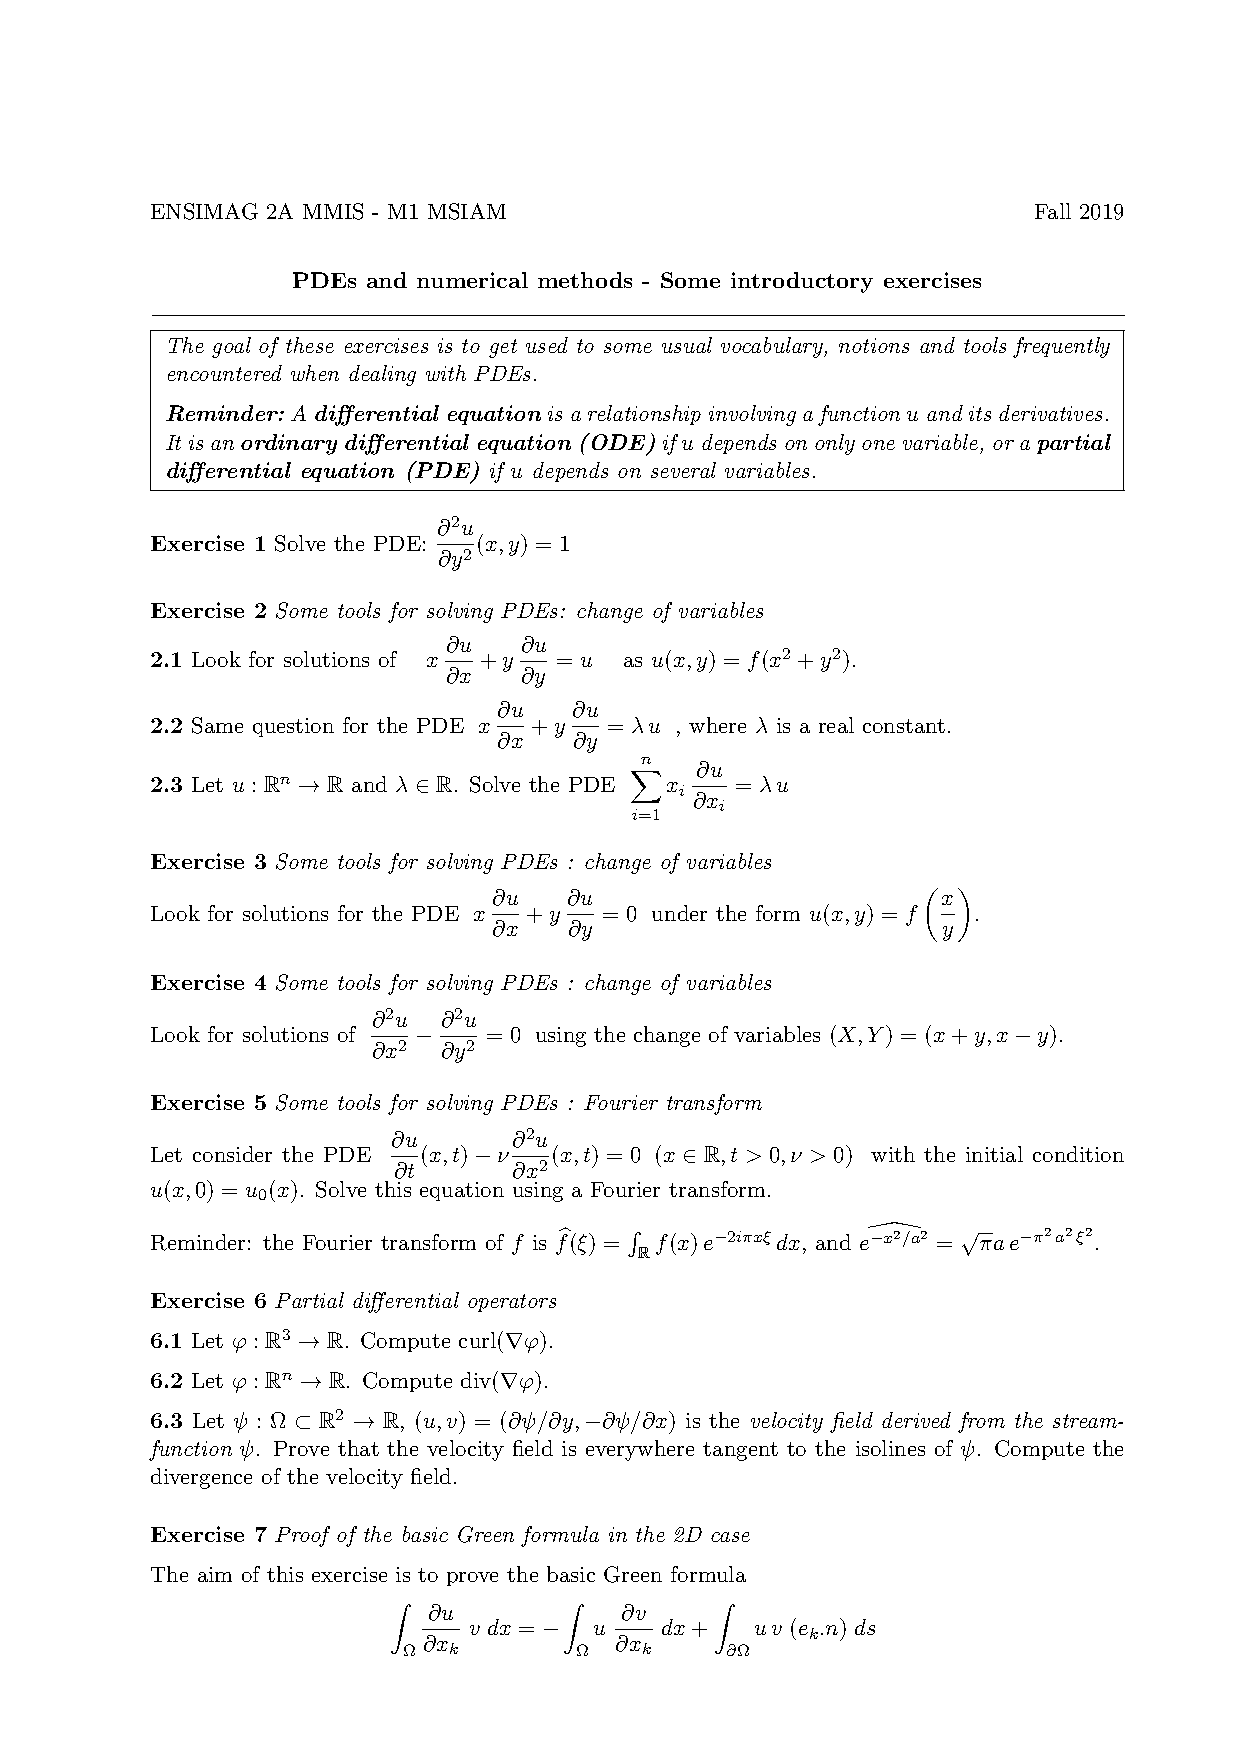
\includepdf[pages=-]{sources/td1.pdf}
\section{Solutions to Problem Set 1}
\label{sec:Solutions to Problem Set 1}
\subsection{Exercise 1}
\label{subsec:Exercise 1}
Solution is simple : 
\begin{align*}
    \frac{ \partial^2 u }{ \partial y^2 } u &= 1 \\ 
    \int\limits_{ }^{ } \frac{ \partial^2 u }{ \partial y^2 } u &= \int\limits_{ }^{ } 1 dy\\ 
    \frac{ \partial u }{ \partial y }  &= y + c(x)  \\ 
    \int\limits_{ }^{ } \frac{ \partial u }{ \partial y } &= \int\limits_{ }^{ } y + c(x)
    dy \\ 
    u &= \frac{ 1 }{ 2 } y^2 + yc(x) + d(x)  \\ 
\end{align*}
\subsection{Exercise 2 : Change of variables }
\label{subsec:Exercise 2 : Change of variables }
\subsubsection{2.1}
Look for solutions of $ x \frac{ \partial u }{ \partial x  } + y \frac{ \partial u  }{
\partial y } = u $ for $ u(x,y) = f(x^2 + y^2) \\ $
First we take the x variable : 
\[
\frac{ \partial u  }{ \partial x } = \frac{ \partial f }{ \partial x } = \left( f'\right)
\left( 2x\right) 
\]
Simlarly for the y variable : 
\[
\frac{ \partial u  }{ \partial y } = \frac{ \partial f }{ \partial y  } = \left( f'
\right) \left( 2y\right) 
\]
Plugging back into the equation : 
\[
2x^2f' + 2y^2f' = f
\]
which can be solved thusly : 
\begin{align*}
    2f' \left( x^2 + y^2 \right) &= f \\
    &\text{Let } x^2 + y^2 = r  \\ 
    \frac{ f' }{ f } &= \frac{ 1 }{ 2 r } \\
    \int\limits_{ }^{ } \frac{ f'  }{ f }  &= \int\limits_{ }^{ } \frac{ 1 }{ 2r }  \\ 
    \ln \left( f\right) &= \frac{ 1 }{ 2 } \ln \left( r\right) + c \\
    f &= e^{\ln(r) / 2 } e^c \\ 
    f &= A\sqrt{r} \quad \text{ where } A = e^c\\ 
\end{align*}
This finally gives us the solution 
\[
    u(x,y) = A\sqrt{x^2 + y^2} \quad A \in \mathbb{R}
\]

\subsubsection{2.2}
Same question for the PDE $ x \frac{ \partial  u }{ \partial x } + y\frac{ \partial u }{
\partial y  }  = \lambda u $ where $ \lambda \in \mathbb{R}  $ and constant.
We begin with the relation 
\[
2rf' = \lambda u 
\]
which gives $ 2rf' = \lambda f $ allowing us to solve. 
\begin{align*}
    2rf'  &= \lambda f \\ 
    \frac{ f' }{ f }  &= \frac{ \lambda  }{ 2r }  \\ 
    \int\limits_{ }^{ } \frac{ f' }{ f } &= \int\limits_{ }^{ } \frac{ \lambda }{ 2r } \\
    \ln\left( f\right)  &= \frac{ \lambda }{ 2 } \ln\left( r\right)  \\ 
    f &= Ar^{ \lambda /  2  } \\ 
\end{align*}
Finally, 
\[
    u(x,y) = A\left( x^2 + y^2 \right) ^{\lambda / 2} 
\]

\subsubsection{2.3}
Let $ u : \mathbb{R} \to \mathbb{R}  $ and $ \lambda \in \mathbb{R}  $. Solve 
\begin{equation}
\sum_{i=1}^{n} x_i \frac{ \partial u }{ \partial x_i } = \lambda u
\label{pr:2.2}
\end{equation}
We first begin with the basic relations 
\[
f(x_1^1 + \cdots + x_n^2) = u(x_1, \cdots , x_n) 
\]
The left hand side of \ref{pr:2.2} elementwise then becomes 
\[
\left( 2x_i^2\right) f'
\] then the entire expression is 
\[
\sum_{i=1}^{n} \left( 2x_i^2 \right) \left( f'\right) = \lambda u
\] then 
\[
\left( 2f'\right) \| x \|^{ 2}_{ } = \lambda f
\] replacing $ \| x \|^{ 2}_{ } = r $ we get 
\begin{align*}
    \frac{ f' }{ f }  &= \frac{ \lambda  }{ 2 } r \\ 
    \ln\left( f\right)  &= \frac{ \lambda  }{ 2 } \ln\left( r\right)  \\ 
    f &= r ^ {\lambda / 2}  \\ 
\end{align*}
So we finally have, 
\[
    \left(  \| x \|^{ 2}_{ } \right) ^ { \lambda / 2} = \|  x \|^{ \lambda }_{ }  
\] 
and our solution is 
\[
u = \| x \|^{ \lambda }_{ } 
\]

\subsubsection{3}
Look for solutions for the PDE $ x \frac{ \partial u }{ \partial x } + y \frac{ \partial u
}{ \partial y } = 0$ under the form $ u(x,y) = f\left( \frac{ x }{ y } \right)  $. 
$ \\ $We first look for x : 
\[
\frac{ \partial f }{ \partial x } = \frac{ f' }{ y }            
\]
for y : 
\[
\frac{ \partial f }{ \partial y } = \frac{ -xf'}{ y^2 } 
\]
Plugging in to the original equation we get
\begin{align*}
    f' \frac{ x }{ y }  - \frac{ x }{ y }f'  &=  0\\ 
    f'\left( \frac{ x }{ y }  - \frac{ x }{ y } \right)  &= 0 \\ 
\end{align*}
which has $ \infty  $ many solutions. 

\subsubsection{Exercise 4}
Look for solutions of $ \frac{ \partial ^2 u  }{ \partial x ^2 } - \frac{ \partial ^2 u }{
\partial y^2 } = 0  $ using $ \left( X, Y\right) = \left( x+y,
x-y\right) . $
\begin{align*}
    \frac{ \partial ^2 f }{ \partial x } - \frac{ \partial^2 f }{ \partial y^2 } = &0\\
\end{align*}
We first compute the left hand side
\begin{align*}
    \frac{ \partial ^2 f  }{ \partial x } &= \frac{ \partial  }{ \partial x } \left(
    \frac{ \partial f }{ \partial x } \right) \\
     &= \frac{ \partial  }{ \partial x } \left( \frac{ \partial f }{ \partial X } \frac{
     \partial X }{ \partial x } + \frac{ \partial f }{ \partial Y } \frac{ \partial Y }{
     \partial x } \right)  \\ 
      &= \frac{ \partial  }{ \partial x } \left( \frac{ \partial f }{ \partial X } +
      \frac{ \partial f }{ \partial Y } \right)  \\ 
\end{align*}

each of these can be a bit tricky. We refer to \ref{th:Chain Rule for Multivariable
Functions} in order to see that 
\begin{align*}
    \frac{ \partial  }{ \partial x } \left( \frac{ \partial f }{ \partial X } \right)  &=
    \frac{ \partial  }{ \partial X } \left( \frac{ \partial f}{ \partial X } \frac{
    \partial X }{ \partial x } + \frac{ \partial f }{ \partial Y } \frac{ \partial Y }{
    \partial x }  \right) \\
     &= \frac{ \partial ^2 f }{ \partial X^2 } \left( 1\right) + \frac{ \partial ^2 f }{
     \partial X \partial Y } \left( 1\right)  \\ 
      &\text{Similarly, for the right hand side}   \\ 
      \frac{ \partial  }{ \partial x } \frac{ \partial f }{ \partial Y }   &= \frac{
      \partial  }{ \partial Y } \left( \frac{ \partial f }{ \partial X } \frac{ \partial x
  }{ \partial x } + \frac{ \partial f }{ \partial Y } \frac{ \partial Y }{ \partial x } \right)  \\
   &= \frac{ \partial ^2 f }{ \partial Y \partial X } \left( 1\right)  + \frac{ \partial^2
   f }{ \partial Y^2 } \left( 1\right)  \\ 
\end{align*}
This leaves us with  
\[
\frac{ \partial ^2 f }{ \partial x^2  } = \frac{ \partial ^2f }{ \partial X^2 } +
\frac{ \partial ^2f }{ \partial X \partial Y } + \frac{ \partial ^2f }{ \partial Y
\partial X } + \frac{ \partial ^2f }{ \partial Y^2 }     
\]
For the second term, 
\begin{align*}
    \frac{ \partial ^2 f }{ \partial y^2  } &= \frac{ \partial  }{ \partial y } \left(
    \frac{ \partial f }{ \partial y } \right) \\
     &= \frac{ \partial  }{ \partial y } \left( \frac{ \partial f }{ \partial X } \frac{
     \partial X }{ \partial x } + \frac{ \partial f }{ \partial Y } \frac{ \partial Y }{
     \partial y } \right)  \\ 
     &= \frac{ \partial  }{ \partial y } \left( \frac{ \partial f }{ \partial X } - \frac{
     \partial f }{ \partial Y } \right)  \\ 
\end{align*}
Thus, 
\begin{align*}
    \frac{ \partial  }{ \partial y } \left( \frac{ \partial f }{ \partial X } \right) &=
    \frac{ \partial  }{ \partial X } \left( \frac{ \partial f }{ \partial X } \frac{
    \partial X }{ \partial y } + \frac{ \partial f }{ \partial Y } \frac{ \partial Y }{
    \partial y } \right) \\
     &= \frac{ \partial  }{ \partial X } \left( \frac{ \partial f }{ \partial X } - \frac{
     \partial f }{ \partial Y }  \right)  \\ 
     &= \frac{ \partial ^2 f }{ \partial X^2 } - \frac{ \partial ^2 f }{ \partial X
     \partial Y }  \\ 
\end{align*}

and, 

\begin{align*}
    \frac{ \partial  }{ \partial y } \left( \frac{ \partial f }{ \partial Y } \right)  &=
    \frac{ \partial  }{ \partial Y } \left( \frac{ \partial f }{ \partial X } \frac{
    \partial X }{ \partial y } + \frac{ \partial f }{ \partial Y } \frac{ \partial Y }{
    \partial y } \right) \\ 
     &= \frac{ \partial  }{ \partial Y } \left( \frac{ \partial f }{ \partial X } - \frac{
     \partial f }{ \partial Y } \right)  \\
      &= \frac{ \partial ^2f }{ \partial Y \partial X } - \frac{ \partial ^2f }{ \partial
      Y^2}  \\ 
\end{align*}

which gives 
\[
\frac{ \partial ^2 f }{ \partial y^2 } =  \frac{ \partial  }{ \partial y } \left( \frac{ \partial f }{ \partial X } \right) - \frac{
\partial  }{ \partial y }\left( \frac{ \partial f }{ \partial Y } \right) = \frac{
\partial ^2f }{ \partial X^2 } - \frac{ \partial ^2 f }{ \partial X \partial Y } - \frac{
\partial ^2 f}{ \partial Y \partial X  } + \frac{ \partial ^2f }{ \partial Y^2 }  
\]
Plugging in to the original equation : 

\[
\frac{ \partial ^2 f }{ \partial x^2  } - \frac{ \partial ^2f }{ \partial y^2 } = 
\frac{ \partial ^2f }{ \partial X^2 } +
\frac{ \partial ^2f }{ \partial X \partial Y } + \frac{ \partial ^2f }{ \partial Y
\partial X } + \frac{ \partial ^2f }{ \partial Y^2 }     
- \left(  \frac{
\partial ^2f }{ \partial X^2 } - \frac{ \partial ^2 f }{ \partial X \partial Y } - \frac{
\partial ^2 f}{ \partial Y \partial X  } + \frac{ \partial ^2f }{ \partial Y^2 }   \right) 
\]
\[
= 0 + 2 \frac{ \partial ^2f }{ \partial X \partial Y } + 2 \frac{ \partial ^2f }{ \partial
Y \partial X} + 0
\]
Assuming mixed partials are equal we get 
\[
\frac{ \partial ^22f }{ \partial X \partial Y } = 0
\]
So we are looking for $ u \in \mathscr{ C } ^2 $ such that the mixed partials are equal to
zero. This gives us the function 
\[ u = F\left( x+y\right) + G\left( x-y\right)  
    \qquad \text{where } F,G \in \mathscr{ C } ^2. 
\]


\subsection{Fourier Transform}
\label{subsec:Fourier Transform}
\begin{equation}
    \frac{ \partial u }{ \partial t } \left( x, t\right) - \nu \frac{ \partial ^2u }{
    \partial x^2 } \left( x,t\right) = 0, \qquad x \in \mathbb{R}, t> 0, \nu > 0 
\end{equation}
With $ u\left( x,0\right) = u_0(x) \\$. 
We want to solve this using the Fourier Transform which we denote using 
\[
    \mathscr{ F } \left( f(x) \right) = \widehat{f}(\xi) = \int\limits_{ \mathbb{R}}^{ }
    f(x) e^{-2i\pi x\xi} \ dx 
\]
Using basic properties of the Fourier Transform we have : 
\[
    \frac{ \partial u }{ \partial t } \widehat{u}(\xi, t) - \nu \left( 2\pi i \xi\right)
    ^2 \widehat{u}(\xi,t) 
\]
\[
    \frac{ \partial u }{ \partial t } \widehat{u}(\xi, t) + \nu4\pi^2\xi^2 \widehat{u}(\xi,t) 
\]
Which gives a seperable equation 
\[
    \int\limits_{ }^{ }  \frac{ du  }{ u } = -\int\limits_{ }^{ } \nu4\pi^2\xi^2 \ dt 
\]
\[
    \widehat{u} = Ae^{-v4\pi^2\xi^2t} \qquad \text{ where } A = e^{cst}
\]
Using initial conditions we have 
\[
    \widehat{u}(\xi, 0) = A = \widehat{u}_0(\xi)
\]
\[
    \widehat{u}(\xi, t) = \widehat{u}_0(\xi)e^{-\nu4\pi^2\xi^2 t}
\]
Using the fact that $ \widehat{e^{-x^2/a}} = \sqrt{\pi} ae^{-\pi^2a^2\xi^2} $, we have : 
\begin{align*}
    \pi^2 a^2 \xi^2  &= \nu 4\pi^2\xi^2 t \\ 
    a^2 &= \nu 4t  \\ 
    a &= 2\sqrt{\nu t}\\
     &\text{ Then, substituting for a }  \\ 
    \mathscr{ F } \left( e _{  }^{ -x^2 / 2\sqrt{\nu t } }\right)  &= 2\sqrt{\pi\nu
    t} e _{  }^{ -\nu4\pi^2  \xi^2 t } \\ 
        \mathscr{ F } \left( \frac{1  }{  2\sqrt{\pi \nu t} } e _{   }^{ -x^2 / 2\sqrt{\nu
        t} }  \right)      &= e _{  }^{ -\nu4\pi^2  \xi^2 t }
\end{align*}
Finally, 
\begin{align*}
    \mathscr{ F } \left( u_0(x)\frac{1  }{  2\sqrt{\pi \nu t} } e _{   }^{ -x^2 / 2\sqrt{\nu
    t} }  \right)      &= u_0(x)e _{  }^{ -\nu4\pi^2  \xi^2 t } 
\end{align*}
\[
u(x,t) &= \frac{ 1 }{ 2\sqrt{\pi\nu t}  } \int\limits_{-\infty}^{\infty} u_0(y) e _{
    }^{ \frac{ -\left( x-y\right) ^2 }{ 4\nu t }  } \ dy \\ 
\]







\subsection{Partial Differential Operators}
\label{subsec:Partial Differential Operators}
\begin{enumerate}
    \item Let $ \varphi : \mathbb{R}^3 \to \mathbb{R} $. Compute curl $ \left( \nabla
        \varphi\right)  $
    \item Let $ \varphi : \mathbb{R}^n \to \mathbb{R} $. Compute div $ \left( \nabla
        \varphi  \right)$
    \item Let $ \psi : \Omega \subset \mathbb{R}^2 \to \mathbb{R} $, $ (u,v) = \left(
        \partial \psi / \partial y, - \partial \psi / \partial x\right)  $
    is the velocitiy field derived from the stream function $ \psi $. Prove that the
    velocity field is everywhere tangent to the isoline of $ \psi $. Compute the
    divergence of the velocity field. 
\end{enumerate}
Using the fact that, for $ \varphi : \mathbb{R}^n \to \mathbb{R}  $ we have that 
\[
            \text{grad } \varphi(\boldsymbol{x}) = \nabla \varphi( \boldsymbol{x} ) = \begin{pmatrix*}
                \frac{ \partial \varphi }{ \partial x_1 }  \\
                 \vdots \\
                 \frac{ \partial \varphi }{ \partial x_n } 
            \end{pmatrix*}
\]


\begin{enumerate}
    \item 
        \begin{align*}
            \text{curl } \varphi(\boldsymbol{x} ) &= \text{curl } \begin{pmatrix*}[r]
                \frac{ \partial \varphi }{ \partial x_1 }   \\[0.5em]
                \frac{ \partial \varphi }{ \partial x_2 }  \\[0.5em]
                 \frac{ \partial \varphi }{ \partial x_3 }  
            \end{pmatrix*}
               \\ 
                &= \begin{pmatrix*}[r]
                    \frac{ \partial ^2 \varphi }{ \partial x_2 \partial x_3 } - \frac{
                    \partial ^2 \varphi }{ \partial x_3 \partial x_2 }   \\[1em] 
                    \frac{ \partial ^2 \varphi }{ \partial x_3 \partial x_1 } - \frac{
                    \partial ^2 \varphi }{ \partial x_1 \partial x_3 }   \\[1em] 
                    \frac{ \partial ^2 \varphi }{ \partial x_1 \partial x_2 } - \frac{
                    \partial ^2 \varphi }{ \partial x_2 \partial x_1 }   \\
                \end{pmatrix*}
                  \\ 
        \end{align*}
    \item   \[\text{div } \varphi(\boldsymbol{x} ) &= \text{curl } \begin{pmatrix*}
                \frac{ \partial \varphi }{ \partial x_1 }   \\[0.5em]
                \vdots  \\[0.5em]
                 \frac{ \partial \varphi }{ \partial x_n }  
            \end{pmatrix*}
        \]
        \[
        = \sum_{i=1}^{n} \frac{ \partial^2 \varphi_i }{ \partial x^2_i } 
        \]
\end{enumerate}

\subsection{Proof of the basic Green Formula in the 2D case}
\label{subsec:Proof of the basic Green Formula in the 2D case}
We want to prove 
\begin{equation}
\int\limits_{\Omega}^{ } \frac{ \partial u }{ \partial x_k } v \ dx = -
\int\limits_{\Omega}^{ } u \frac{ \partial v  }{ \partial  x_k  } \ dx + \int\limits_{
\partial \Omega } uv \left( e_k \cdot n \right) \ ds
\label{eq:general_green_formula}
\end{equation}
where $ e_k $ is the unit vector in direction $ x_k $, in the 2D-case $ \left( \Omega
\subset \mathbb{R} \right)  $.

\begin{figure}[ht]
    \centering
    \incfig{greenonomega}
    \caption{greenOnOmega}
    \label{fig:greenonomega}
\end{figure}

\newpage 
\subsubsection{7.1}
Prove this formula for $ \Omega  $ being the reference triangle (i.e, with nodes $ \left(
0,0\right) , \left( 1,0\right) , \left( 0,1\right)  $). 
\begin{figure}[ht]
    \centering
    \incfig{green-on-t}
    \caption{green on T}
    \label{fig:green-on-t}
\end{figure}
 
The left hand side of \ref{eq:general_green_formula} becomes 
\[
\int\limits_{\Omega}^{ } \frac{ \partial u }{ \partial x_1 } v \ dx_1 dx_2 
\] or 
\begin{align*}
    \int\limits_{T}^{ } \frac{ \partial u }{ \partial x_1 } v\ dx_1dx_2  &= 
    \int\limits_{x_1 = 0}^{1} \left( \int\limits_{x_2 = 0}^{x_2= 1
    - x_1 } \frac{ \partial u }{ \partial x_1 } v \ dx_2\right) dx_1 \\
     &= \int\limits_{x_2 = 0}^{1} \left( \int\limits_{x_1 = 0}^{1 - x_2} \frac{ \partial u
     }{ \partial x_1 } v \ dx_1\right) dx_2 \\ 
\end{align*}
The last formulation has a fixed $ x_2 $ for the inner part of the equation. 

\begin{prop}[]
    \[
        \int\limits_{ \partial \Omega} f \ d\sigma = \sum_{i=1}^{m} \int\limits_{ \partial
        \Omega_i }^{ } f \ d\sigma 
    \]
    That is, each side of the boundary can be analyzed independently for simple
    parametrization, furthermore, the combination of the pieces is that integral of the
    entire boundary. $ \\ $
    We get the following formation due to the defintion of a line integral :  
    \[
        \int\limits_{ \partial \Omega} f \ d\sigma = \int\limits_{0}^{1} f\left(
        \gamma_i(t) \right) \| \gamma'_i(t) \|^{ }_{ } \ dt 
    \]
\end{prop}

Furthermore, we calculate the unit normal for each segment of the triangle. 
\[
\partial T_1 = \begin{pmatrix*}[r]
    0 \\
    0 
\end{pmatrix*}
- \begin{pmatrix*}[r]
     1 \\
     0 
\end{pmatrix*}
 = \begin{pmatrix*}[r]
      -1 \\
      0 
 \end{pmatrix*}
 \text{ which has normal } n_1 = \begin{pmatrix*}[r]
     0  \\
     -1 
 \end{pmatrix*}
 
\] 

\[
\partial T_2 = \begin{pmatrix*}[r]
     1 \\
     0 
\end{pmatrix*}
- \begin{pmatrix*}[r]
    0 \\
    1 
\end{pmatrix*}
= \begin{pmatrix*}[r]
     1 \\
    -1 
\end{pmatrix*}
\text{ which has length } \| \cdot  \|^{ }_{ } = \sqrt{2}
\]
thus, 
\[
\begin{pmatrix*}[r]
     1 \\
     -1 
\end{pmatrix*}
\cdot \begin{pmatrix*}[r]
     1 \\
     1 
\end{pmatrix*}
= 0 , 
\]
 and we divide by the length to ensure the normal has length 1
\[
\partial T_2 = \begin{pmatrix*}[r]
    \frac{ 1 }{ \sqrt{2}} \\[0.5em]
    \frac{ 1 }{ \sqrt{2} }  
\end{pmatrix*}
\]
The last is found simply, 
\[
\partial T_3 = \begin{pmatrix*}[r]
    -1 \\
     0
\end{pmatrix*}
\]
We can now solve for each side. 

\[
    \int\limits_{x_2=0}^{1} \left( - \int\limits_{x_1=0}^{1-x_2} u \frac{ \partial v  }{
    \partial x_1 } \right) \ dx_2 +  \int\limits_{x_2=0}^{1} u\left( 1-x_2, x_2\right)
    v\left( 1-x_2, x_2\right) - u\left( 0,x_2\right) v\left( 0,x_2\right) \ dx_2
\]
\begin{align*}
    \int\limits_{ \partial T}^{ } uvn_1 \ d\sigma &= \int\limits_{ \partial
    T_1}^{ } uv\overbrace{ n_1}^{=0} \ d\sigma + \int\limits_{ \partial T_2 }^{ }
    uv\overbrace{n_1}^{=1/\sqrt{2}} + \int\limits_{ \partial T_3}^{ }
    uv\overbrace{n_1}^{=-1} \ d \sigma \\
     &= \int\limits_{ \partial T_2}^{} uvn_1 \ d\sigma + \int\limits_{ \partial T_3}^{ }
     uvn_1 \ d\sigma   \\ 
\end{align*}
Now, for $ \partial T_2 $ we have the paramaterized line as 
\[
    \gamma_2 (t) = \set{ \left( 1-t, t\right) , t\in [0,1] } \text{ where } \gamma_2'(t) =
    \begin{pmatrix*}[r]
        -1 \\
         1 
    \end{pmatrix*}
    \text{ and } 
    \| \gamma_2' \|^{ }_{ } = \sqrt{2}
\]
Finally, 
\[
    \int\limits_{0}^{1} u\left( 1-t, t\right) v\left( 1-t, t\right) \frac{ 1 }{ \sqrt{2} }
    \sqrt{2} \ dt 
\]
Since $ \gamma_3(t) = \set{ \left( 0, 1-t\right)  }  $ we have 
\[
    \int\limits_{0}^{1} u\left( 0,t\right) v\left( 0,t\right) (-1) \cdot (1) \ dt
\]
and 
\[
\int\limits_{0}^{1} u\left( 1-t, t\right) v\left( 1-t, t\right) -  u\left( 0,t\right) 
v\left( 0,t\right) \ dt
\]

\subsection{Green Formulas}
\label{subsec:Green Formulas}
\begin{enumerate}
    \item \[
            \int\limits_{\Omega}^{ } \text{div}\left( \boldsymbol{E} (\boldsymbol{x})
            \right) \ d\boldsymbol{x} \quad \text{ with } \boldsymbol{E} : \Omega \subset
            \mathbb{R}^n \to \mathbb{R}^n
    \]
First, it should be noted that the div of a function is a scalar, and we take u = 1. Thus, 
\begin{align*}
    \int\limits_{\Omega}^{ } u \text{ div}(\boldsymbol{E}) \ dx &= - \int\limits_{\Omega}^{ }
    \underbrace{\nabla u}_{=0} \cdot \boldsymbol{E} + \int\limits_{ \partial \Omega }^{ } u \left(
\boldsymbol{E} \cdot \boldsymbol{n} \right) \ ds \\
 &= \int\limits_{ \partial \Omega} u \left( \boldsymbol{E} \cdot \boldsymbol{n}  \right) \
 ds\\ 
 &\text{ since } u = 1\\
    \int\limits_{\Omega}^{ } \text{div} \left( \boldsymbol{E} \right) \ dx &= \int\limits_{
 \partial \Omega}^{ } \boldsymbol{E} \cdot \boldsymbol{n} \ ds 
\end{align*}

\item \[
        \int\limits_{\Omega}^{ } \text{div}\left( k(\boldsymbol{x}) \nabla
        u(\boldsymbol{x})   \right) \ d\boldsymbol{x} 
        \quad \text{ with } u : \Omega \subset \mathbb{R}^n\to \mathbb{R}
\]
\begin{align*}
    \int\limits_{\Omega}^{ } \text{div}\left( k(\boldsymbol{x} ) \nabla u(\boldsymbol{x} )
    \right) \ d\boldsymbol{x}   &=  \\ 
\end{align*}

\item 
    \[
    \int\limits_{\Omega}^{} \sum_{i=1}^{n} \alpha_i \frac{ \partial u }{ \partial x_i }
    \frac{ \partial v  }{ \partial x_i } \quad \text{ with } u,v : \Omega \subset
    \mathbb{R}^n \to \mathbb{R} \text{ and } \alpha_i \in \mathbb{R} 
    \]
\end{enumerate}


\subsection{Boundary conditions and well-posedness}
\label{subsec:Boundary conditions and well-posedness}

\subsubsection{9.1}
Let the ODE 
\[
    u''(x) = 0 \text{ in } ]a,b[
\]
Find its solution considering 
\begin{enumerate}[label={(\alph*)}]
    \item Dirichlet Conditions : $ u(a) = \alpha, \ u(b) = \beta $
    \item Neumann conditions : $ u'(a) = \alpha , \ u'(b) = \beta  $
    \item Robin conditions : $ u'(a) + \lambda u(a) = \alpha, \ u'(b) + \lambda u(b) =
        \beta  $ with $ \lambda \neq 0 $
    \item Mixed conditions : $ u'(a) = \alpha $, $ u(b) = \beta $
\end{enumerate}
We begin with the fact that this ODE has the general form of 
\[
    u(x) = Ax + B
\]
\begin{enumerate}[label={(\alph*)}]
    \item This gives us the condition that 
        \[
            u(a) = Aa + B = \alpha \qquad u(b) = Ab + B = \beta 
        \]
        Intuitively, this is well posed because there exists a unique line between two
        points. In terms of a solution we get : 
        \[
            A = \frac{ \beta - \alpha  }{ b - a } \qquad B = \alpha - \frac{ \beta -\alpha
            }{ b-a } (a) 
        \]
    \item Since $ u'(x) = A = \alpha = \beta $ which does not guarantee uniqueness. 
    \item 
        \[
            A + \lambda \left(Aa + B  \right) = \alpha \qquad A + \lambda \left( Ab + B\right)  = \beta 
        \] which gives us 
        \[
            A\left( 1 + \lambda a\right) + \lambda B = \alpha \qquad A\left( 1 + \lambda
            b\right) + \lambda B = \beta 
        \]
        we can test linear dependence via the determinate, which gives 
        \[
        \lambda\left( 1 + \lambda a\right) - \lambda\left( 1 + \lambda B\right) =
        \lambda^2\left( a-b\right) \neq 0
        \]
    \item The last conditions give : 
        \[
        u'(a) = \alpha \implies A = \alpha \qquad \text{ then } u(b) = \alpha b + B
        \implies B = \beta - \alpha b
        \] 
        This solution is unique since it depends on both endpoints. 
\end{enumerate}


\subsubsection{9.2}
Consider 
\begin{equation}
    \triangle u = f \quad \text{ on } \Omega \subset \mathbb{R}^n
    \label{eq:9.2}
\end{equation}
\begin{enumerate}[label={(\alph*)}]
    \item Dirichlet conditions : $ u = g  $ on $ \partial \Omega  $
    \item Neumann conditions : $ \frac{ \partial u }{ \partial n  } = h $ on $ \partial
        \Omega $
    \item Mixed conditions : 
        \[
        u = g \text{ on } \Gamma_0, \quad \frac{ \partial u }{ \partial n  } = h \text{ on
        } \Gamma_1, \text{ where } \Gamma_0 \cup \Gamma_1 = \partial \Omega \text{ and }
        \Gamma_0 \cap \Gamma_1 = \emptyset 
        \]
\end{enumerate}
(a) 
We use the approach of assuming that there can be two solutions which result in a
contradiction. Let $ u_1,u_2 $ be two solutions of $ \triangle u = f \text{ on } \Omega $.
We then have 
\[
    \begin{aligned} 
&\begin{cases} 
    \begin{aligned}
        \triangle u_1 &= f \text{ in } \Omega \qquad \\
        u_1 &= g \text{ on } \partial \Omega 
    \end{aligned}
\end{cases}
&\begin{cases} 
    \begin{aligned}
        \triangle u_2 &= f \text{ in } \Omega \qquad \\
        u_2 &= g \text{ on } \partial \Omega 
    \end{aligned}
\end{cases}
\end{aligned} 
\]
If $ u_1,u_2 $ solutions then $ u = u_1 - u_2  $ is a solution 
\[
\begin{cases}
    \begin{aligned}
        \triangle u &= f - f = 0 \quad &\text{ in } &\Omega   \\ 
        u &= g - g = 0 \quad &\text{ on } &\partial   \Omega   \\ 
    \end{aligned} 
\end{cases}
\]

Using Green's theorem we get : 
\begin{align*}
    \int\limits_{\Omega}^{ } \triangle u v \ dx &= - \int\limits_{\Omega}^{ } \triangle u
    \triangle v \ dx + \int\limits_{ \partial \Omega }^{ } \partial _nuv \ d\sigma \\ 
     &\text{Where } \partial _nu \text{ or } \frac{ \partial u }{ \partial n  } = \nabla
     u\cdot n \text{ or } \sum_{}^{} \frac{ \partial u }{ \partial x_k }   \\ 
      &\text{Can be found in the class slides}  \\ 
      &= \int\limits_{\Omega}^{ } \underbrace{\triangle u}_{=0} v \ dx - \int\limits_{
      \partial \Omega }^{ } \underbrace{ \nabla u \nabla v }_{=0} \ dx =
      \int\limits_{\Omega}^{ } \frac{ \partial u }{ \partial n  } \underbrace{u}_{=0} \
      d\sigma \\ 
\end{align*}
Assuming smoothnes, this implies that $ \nabla u = 0  $ in $ \Omega $ and $ u $ is
constant on $ \Omega $ where $ \Omega $ is simply connected or, for each component of $
\Omega  $ $ u $ is constant on it. But this is in contradiction with our assumption that 
\[
\triangle u = f
\]Therefore $ u_1 = u_2 $. 

$ \\ $
b) Neuman   
$ \\ $

\begin{equation}
    \partial _n u = h \qquad \text{ on } \partial \Omega 
    \label{eq:neuman_condition}
\end{equation}


Let $ u_1, u_2 $ be solutions of \ref{eq:9.2} and \ref{eq:neuman_condition} and $ u = u_1
-u_2$.
\[
\begin{cases}
    \triangle u  &= 0 \qquad \text{ in } \Omega \\
    \partial _n u &= 0 \qquad \text{ on } \partial \Omega \\ 
\end{cases}
\]
Then, 
\[
\int\limits_{ \partial \Omega}^{ } u \partial _n u \ d\sigma = 0
\]
Thus, $ \nabla u=0   $ in $ \Omega $ and $ u = cst  $ on each connected component of $
\Omega $. which verifies $ \partial _n u = 0 $ on $ \partial \Omega $. No "uniqueness" but
"uniqueness up to a constant." 

$ \\ $
c) 
$ \\ $
\begin{equation}
    \begin{cases}
        u &= g \text{ on } \Gamma_0 \\
        \partial _n u &=h \text{ on } \Gamma_1
    \end{cases}
    \label{eq:robin_conditions}
\end{equation}
Let $ u_1, u_2 $ be solutions of \ref{eq:9.2} \ref{eq:robin_conditions} then $ u = u_1 -
u_2  $ verifies 
\[
\begin{cases}
    \nabla u  &= 0 \text{ in } \Omega \\
    u &= 0 \text{ on } \Gamma_0 \\ 
    \partial _n u &= 0 \text{ on } \Gamma_1 \\ 
\end{cases}
\]
and we have the formula 
\[
\int\limits_{ \partial \Omega}^{ } \partial _n u u \ d\sigma = \int\limits_{\Gamma_0}^{ }
\partial _nu \underbrace{u \ d\sigma}_{=0} + \int\limits_{\Gamma_1}^{ } \partial _n u \ u
\ d\sigma 
\]

If $ \Omega  $ is connected, as $ u = 0 $ on $ \Gamma_0 $, if the measure of $ \Gamma_0 $
is greater than 0 then $ u \equiv 0 $ in $ \Omega $. 




























\chapter{Bezier Curves} 
Invented by Pierre Bezier (Renault) and Pierre De Casteljau (Citreon). 
No interpolation points, rather we have "control points". 

\section{Bernstein Polynomials}
\label{sec:Bernstein Polynomials}
\begin{defn}[Bernstein Polynomials]
    $ \\ $
    Let $ n \in \mathbb{N}  $ and $ i \in \set{ 0, \dots, n  }  $. Then the Bernstein
    polynomials are given by 
    \[
        B^n_i(t) = \begin{pmatrix*}
             n \\
             i 
        \end{pmatrix*}
        t^i \left( 1 - t\right) _{  }^{ n-i } 
    \] where 
    \[
    \begin{pmatrix*}
         n \\
         i 
    \end{pmatrix*}
    = \frac{ n! }{ i! \left( n - i\right) ! } 
    \]
    \label{def:bernsteinPoly}
\end{defn}
\subsection{Properties}
\label{subsec:Properties}
\begin{enumerate}[label={(\alph*)}]
    \item Positivity : 
        \[
            \forall i \ B^n_i(t) \geq 0
        \]
    \item Partition of unity : 
        \[
            \sum_{i=0}^{n} B^n_i (t) = 1
        \]
    \item Linear precision : 
        \[
            \sum_{i=0}^{n} \frac{ i }{ n  } B^n_i(t) = t
        \]
    \item Recursion Formula : for $ 0 \leq i \leq n $
        \[
            B^n_i(t) = \left( 1-t\right) B _{ i }^{ n-1 } (t) + B _{ i-1 }^{ n-1 } (t) 
        \]
        with the convention that $ B _{ j }^{ n  } = 0  $ if $ j \notin [0,n] $
    \item Symmetry : 
        \[
        B _{ i }^{ n  } = B _{ n- i  }^{ n  } \left( 1-t \right) 
        \]
    \item Derivative : 
        \[
            B _{ i }^{ n  } '(t) = n \left( B _{ i-1  }^{ n-1 } (t) - B _{ i }^{ n-1 } (t) \right) 
        \]
    \item Extremum : 
        $ \\ B _{ i }^{ n   } $ has an extremum at $ t = \frac{ i }{ n  }  $
    \item Basis : 
        \[
            \set{ B _{ i }^{ n  } , 0\leq i \leq n  } \text{ is a basis of }
            \mathbb{R}_n[x]
        \]
\end{enumerate}

\subsubsection{a) }
ok 

\subsubsection{b)}
\[
    \sum_{i=0}^{n} B _{ i }^{ n } = \sum_{i=0}^{n} 
    \begin{pmatrix*}
        n \\
        i 
    \end{pmatrix*}
    t^i\left( 1 - t\right) ^{n-i} 
\]
Using the binomial theorem, which states that 
\[
    \left( a+b\right) ^n
\sum_{i=0}^{n} \begin{pmatrix*}
    n \\
    i 
\end{pmatrix*}
a^ib^{n-i} 
\] 
Therefore, we have 
\[
\left( t + \left( 1 - t\right) \right) ^n = 1
\]


\subsubsection{c)}
?


\subsubsection{d)}
We have, from definition of binomial that 
\[
\begin{pmatrix*}
     n \\
     i-1
\end{pmatrix*}
+ 
\begin{pmatrix*}
     n \\
     i
\end{pmatrix*}
=
\begin{pmatrix*}
    n+1  \\
    i  
\end{pmatrix*}
\]

Expanding the original equation and simplifying the coefficents. 

\[
\begin{pmatrix*}
    n   \\
    i  
\end{pmatrix*}
t^i\left( 1-t\right) _{  }^{ n-i } = \begin{pmatrix*}
    n-1  \\
    i  
\end{pmatrix*}
t^i\left( 1-t\right) _{  }^{ n-i } + \begin{pmatrix*}
    n-1  \\
    i-1  
\end{pmatrix*}
t^{i}\left( 1-t\right) ^{n-i} 
\]
We now have 
\begin{align*}
    &\left( \begin{pmatrix*}
        n-1  \\
        i-1  
    \end{pmatrix*}
    + 
    \begin{pmatrix*}
        n-1  \\
        i  
    \end{pmatrix*}
\right) t^i\left( 1-t^{n-i} \right) \\
 &= \begin{pmatrix*}
     n   \\
     i  
 \end{pmatrix*}
 t^i\left( 1-t\right) ^{n-i}   \\ 
 &= B _{ i }^{ n  } (t) \\ 
\end{align*}

\subsubsection{e) }
We have from properties of binomials that 
\[
\begin{pmatrix*}
    n   \\
    k  
\end{pmatrix*}
= \begin{pmatrix*}
    n   \\
    n-k  
\end{pmatrix*}

\]
Then 
\begin{align*}
    B _{ n-i }^{ n } \left( 1 - t\right) &= 
\begin{pmatrix*}
     n \\
     n-i  
\end{pmatrix*}
\left( 1-t\right) ^{n-i} \left( 1-(t-1)\right) ^{ n - (n-i)} \\
                                         &= \begin{pmatrix*}
                                             n   \\
                                             i  
                                         \end{pmatrix*}
                                         t^i \left( 1-t\right) _{  }^{ n-i } 
\end{align*}

\subsubsection{f)}
\[
    n \left( B _{ i-1 }^{ n-1 } (t) - B _{ i }^{ n-1 } (t)\right) 
\]
\[
= n \begin{pmatrix*}
     n-1 \\
     i-1 
\end{pmatrix*}
t^{i-1} \left( 1-t\right) ^{n-i} - n \begin{pmatrix*}
    n-1 \\
     i 
\end{pmatrix*}
t^i \left( 1-t\right) ^{n-1-i} 
\]
\[
= i \begin{pmatrix*}
     n \\
     i 
\end{pmatrix*}
t^{i-1} \left( 1-t\right) ^{n-i} -  \begin{pmatrix*}
    n \\
     i 
\end{pmatrix*}\left( n-i \right) 
t^i \left( 1-t\right) ^{n-1-i} 
\]
\[
=  \begin{pmatrix*}
     n \\
     i 
\end{pmatrix*}
t^{i-1} \left( 1-t\right) ^{n-1-i} 
\left( i\left( 1-t\right) - \left( n-i\right) t\right)          
\]
\[
= \begin{pmatrix*}
    n  \\
    i 
\end{pmatrix*}
t ^{i-1} \left( 1-t\right) ^{n-1-i} \left( i-tn \right) 
\]
On the other hand 
\[
    B' _{ i }^{ n  } (t) = \begin{pmatrix*}
         n \\
         i 
    \end{pmatrix*}
    \left( it^{i-1} \left( 1-t \right) ^{n-i} - t^i \left( 1-t\right) ^{n-i-1} \left(
    n-i\right) \right) 
\]
\[
= \begin{pmatrix*}
     n \\
     i 
\end{pmatrix*}
t^{i-1} \left( 1-t\right) ^{n-1-i} \left( i\left( 1-t\right) -t\left( n-i\right) \right) 
\]

\section{Bezier Curves}
\label{sec:Bezier Curves}
\subsection{Refresher on Convex Hull and Barycenter}
\label{subsec:Refresher on Convex Hull}
\begin{prop}[]
    Let $ p_1, \cdots, P_n \in \mathbb{R}^d $ and $ \lambda_1, \cdots , \lambda_n \in
    \mathbb{R} $ and $ \sum_{i=1}^{n} \lambda_i \neq 0 $
    \[
    \exists ! \in \mathbb{R}^d , \sum_{i=0}^{n} \lambda_i \boldsymbol{GP} _i =
    \boldsymbol{0} 
    \]
    G is given by 
    \[
    \boldsymbol{OG} = \frac{ \sum_{i=1}^{n} \lambda_i \boldsymbol{OP} _i }{ \sum_{i=1}^{n}
    \lambda_i } 
    \]
    G is called the barycenter of $ P_i $ with weight $ \lambda_i $
    \label{prop:}
\end{prop}
\begin{proof}
    Let $ o \in \mathbb{R}^d  $ be any point 
    \begin{align*}
        \boldsymbol{o}  &= \sum_{i=1}^{n} \lambda_i \boldsymbol{GP} _i = \sum_{i=1}^{n}
        \lambda_i\left( \boldsymbol{GO} + \boldsymbol{OP_i} \right)   \\ 
         &= \left( \sum_{i=1}^{n} \lambda_i\right) \boldsymbol{GO} +
         \sum_{i=1}^{n}\lambda_i \boldsymbol{OP_i}   \\ 
    \end{align*}
    
\end{proof}


\begin{defn}[Convec Set]
    $ K \subset \mathbb{R}^d $ is convex if 
    \[
        \forall x,y \in K, \quad [x,y] \subset K
    \]
    \label{def:Convec Set}
\end{defn}

\begin{defn}[Convex Hull]
    Denoted 
    \[
        \text{Conv}\left( K\right) = \cap_{K \subset K'} K' 
    \]
    The smallest convex set that contains the set
    \label{def:Convex Hull}
\end{defn}

\begin{prop}[]
    $ A = \set{ p_1, \cdots, p_n }  $ then 
    \[
    \text{Conv } \left( A\right) = \set{ \sum_{i=1}^{n} \lambda_ip_i, \sum_{i=1}^{n}
    \lambda_i = 1, \ \lambda_i \geq 0 } 
    \]
    is the set of barycenter with positive weights
    \label{prop:}
\end{prop}

\begin{proof}
    Let 
    \[
    F = \set{ \sum_{}^{} \lambda_ip_i, \sum_{}^{} \lambda_i = 1, \lambda_i \geq 0 } 
    \]
    Conv $ (A) \subset F $, F convex. 
    \begin{align*}
        m \in F &\implies m = \sum_{}^{} \lambda_ip_i  \\ 
        n \in F &\implies m = \sum_{}^{} \lambda_i'p_i  \\ 
    \end{align*}
    \[
        q \in [m,n] \implies q = tm + (1-t)n \ t\in [0,1]
    \]

    So 
    \[
        q = \sum_{i=1}^{n} \underbrace{\left( t\lambda_i + \left( 1-t\right)
            \lambda_i'\right)  }_{\lambda_i'' \geq 0}p_i \in F
    \] 
    Then $ [m,n] \subset F $. $ F\subset A $ and $ \lambda''_i = 1 $

    $ \\ $
    $ F \subset \text{Conv}(A) $
    By recursion $ P(n) : $ every barycenter of n points $ q_1, \cdots, q_n  $ belong to
    Conv($q_1, \cdots, q_n)  $. $ \\ $
    n = 1 : 
    $ \\ $
    Let $ n \geq 1  $ $ Sq P(n) $ 
    $ \\ $
    Let $ p_1, \cdots, p_{n+1}  $ points of $ \mathbb{R}^d $ and $ \lambda_1, \cdots,
    \lambda_{n+1} \in \mathbb{R}^d $ with sum = 1. and 
    \[
        m = \sum_{i=1}^{n+1} \lambda_ip_i = \sum_{i-1}^{n} \lambda_ip_i +
        \lambda_{n+1}p_{n+1} + 1
    \]
    Let $ g $ denote the barycenter of $ p_1, \cdots, p_n  $ with associated $ \lamda_i  $
    then 
    \[
    \sum_{i=1}^{n} \lambda_ip_i = \left( \sum_{i=1}^{n} \lamda_i\right) g
    \]
    \[
        = \left( 1-\lambda_{n+1} \right) g
    \]
    then 
    \[
        m = \left( 1-\lambda_{n+1}\right) g + \lambda_{n+1}p_{n+1} \in [g, p_{n+1} ] 
    \]
    by assumption $ g\in \text{Conv}\left( A\right)  \implies m \in \text{Conv}\left(
    A\right)   $.

\end{proof}

\begin{exmp}[]
    \[
        [p_1, p_2] = \set{ tp_1 + \left( 1-t\right) p_2, t\in [0,1] } 
    \]
\end{exmp}



\begin{defn}[]
    We see $ \mathbb{R}^d $ is both affine and vector space. 
    \begin{itemize}
      \item $ p\in \mathbb{R}^d $ is a point 
      \item $ p-q = \boldsymbol{pq}  $ is a vector  
  \end{itemize}
    \label{def:}
\end{defn}

In particular $ \sum_{i=1}^{n} \lambda_ip_i = 0 $ gives a vector, barycenter otherwise(a
point). 


\subsection{Definition of Bezier Curves}
\label{subsec:Definition of Bezier Curves}
Let $ p_0, \cdots, p_n $ points of $ \mathbb{R}^d,\ n > 0 $. The Bezier curve associated
to $ p_0, \cdots, p_n $ is the parametrized curve
\begin{align*}
    P:[0,1] &\rightarrow \mathbb{R}^d  \\ 
    t &\rightarrow \sum_{i=0}^{n} P_iB_i^n(t)
\end{align*}
We call $ [P_o, \cdots, P_n] $ the Bezier control polygon. 

\begin{exmp}[n=1]
    \[
        P(t) = p_0B _{0 }^{ 1 }(t) + B _{ 1 }^{ 1 } (t) 
    \]
    \[
    = p_0t + p_1\left( 1-t\right) 
    \]
    P is a parametrization of $ [p_0, p_1] $
\end{exmp}


\subsection{Properties}
\label{subsec:Properties}
\begin{enumerate}[label={(\alph*)}]
    \item boundary : 
        \[
            P(0) = P_0 \qquad \text{ and } P(1) = P_n
        \]
        \begin{proof}
            \[
                P(0) = \sum_{i=0}^{n} B _{ i }^{ n  } (0)P_i = P_0 
            \]
        \end{proof}
    \item Convex Hull : 
        \[
            P\left( [0,1]\right) \subset \text{Conv}\left( \text{control polygon} \right)  
        \]
        \begin{proof}
            $ \forall t \in [0,1] $ $ P(t) = \sum_{i=0}^{n} B _{ i }^{ n }(t) P_i   $
            where $ B _{ i }^{ n  }  $ is $ \lambda_i  $ which is positive and the sum of
            which is equal to one. Therefore, P belongs to the convex hull. 
        \end{proof}
\newpage
        \begin{figure}[ht]
    \centering
    \incfig{convex-hull}
    \caption{A convex set (red) and its Hull (pink)}
    \label{fig:convex-hull}
\end{figure}



    \item Affine Invariance : 
        Let $ P_1, \cdots, P_n $ and $ f: \mathbb{R}^d \to \mathbb{R}^d $ affine
        transformation. The result is the same if 
        \begin{enumerate}
            \item \[
                    Q(t) = \sum_{i=0}^{n} B _{ i }^{ n  } (t)P_i \rightsquigarrow f
                    \circ Q 
            \]
        \item $\widetilde{Q}(t) = \sum_{}^{} B _{ i }^{ n }(t)f(P_i) $
        \end{enumerate}
        This just simply says that moving the polygon using an affine transformation gives
        us the exact same curve. 

    \item Reduction of Variation
        \begin{prop}[]
            The Bezier curve has less intersection points with any line than its control
            polygon. 
            For any line, the number of intersections between the curve 
            less that the number of intersections between the polygon and 
        \end{prop}
        \begin{proof}
            Admitted. 
        \end{proof}
\begin{figure}[ht]
    \centering
    \incfig{variance-reduction}
    \caption{Variance Reduction}
    \label{fig:variance-reduction}
\end{figure}
    \item Matrix Representation : 
        \begin{align*}
            P(t) &= \sum_{i=0}^{n} B _{ i }^{ n  } (t) P_i  \qquad t\in [0,1]\\
        \end{align*}
        can be done as a scalar product between vector with Bernstein polynomials where
        each line is for a point $ t_i $ and the vector is the points $ P_0, \cdots, P_n $
        \[
            P(t_ = [P_0, \cdots, P_n] \begin{pmatrix*}
                B _{ 0 }^{ n  } (t) \\
                \vdots \\
                B _{ n  }^{ n  } (t) 
            \end{pmatrix*}
        \]
        Matrix of change of Basic 
        \[
        Q\coloneqq \begin{pmatrix*}
            B _{ 0 }^{ n  }& \cdots& B _{ n  }^{ n  }  \\
              \
        \end{pmatrix*}
        
        \]
        \[
            B _{ i }^{ n  } (t) = \sum_{i=0}^{n} q_i0
        \]
        Then 
        \[
        \begin{pmatrix*}
            B _{ 0 }^{ n  }   \\
            \vdots \\
            B _{ n  }^{ n  } 
        \end{pmatrix*}
        = Q^T \begin{pmatrix*}
            1  \\
            \vdots \\
            t^n
        \end{pmatrix*}
        
        \]
        then 
        \[
            P(t) = \underbrace{[P_0, \vdots, P_n ]^tQ }_{Q_0, \cdots, Q_n] \begin{pmatrix*}
                1  \\
                \vdots \\
                t^n
            \end{pmatrix*}
            
        \]
        \begin{prop}[]
            \[
                [P_0, \cdots, P_n] = Q^T[Q_0, \cdots, Q_n] 
            \]
            Where P... is the control polygon in the bernstein basis, and $ Q^T $ is the
            transpose and expression in the monomial basis
            \label{def:}
        \end{prop}

    \item Derivative of Bezier Curves 
        \begin{prop}[]
            \[
                P'(t) = n \sum_{i=0}^{n-1} \underbrace{\left( P_{i+1} - P_i
                \right)}_{\Delta P_i = \frac{ P_{i+1} - P_i }{ \left( i+1\right) - i } } B _{ i }^{ n-1 }
                (t) 
            \]
            \label{def:}
        \end{prop}
        \begin{proof}
            \begin{align*}
                P'(t) &= \sum_{i=0}^{n} P_i B _{ i }^{ n  } '(t) \\
                      &= \sum_{i=0}^{n} P_in \left( B _{ i-1 }^{ n-1 } (t) - B _{ i }^{
                      n-1 } (t)\right)  \\ 
                      &= n \left(\sum_{i=0}^{n-1} P_{i+1} B _{ i  }^{ n-1  } (t) -
                      \sum_{i=0}^{n-1} P_i B _{ i }^{ n-1 } (t) \right)  \\ 
                      &= n \sum_{i=0}^{n-1} \left( P_{i+1} - P_i \right) B _{ i }^{ n-1 }
                      (t)\\ 
            \end{align*} 
        \end{proof}
        $ P' $ is a Bezier curve Associated to $ [n\Delta P_0, \cdots , n\Delta P_{n-1}] $
        Similarly, one has 
        \begin{prop}[]
            \[
                P''(t) = n\left( n-1\right) \sum_{i=0}^{n-2} \Delta^2P_i B _{ i }^{ n-2 }
                (t) 
            \]
            Where $ \Delta^2 P_i = \Delta P_{i+1} - \Delta P_i  = P_{i+2} - 2P_{i+1] + P_i$
            \label{def:}
        \end{prop}
        Also : 
        \[
            P _{  }^{ (k) } (t) = \frac{ n! }{ \left( n-k\right) ! } \sum_{i=0}^{n-k}
            \Delta^k P_i B _{ i }^{ n-k } (t) 
        \]
        Where $ \Delta^k P_i  $ are defined recursively. 
        $ \\ $
        In particular : 
        \begin{align*}
            P'(0)  &= n\Delta P_0 = n \boldsymbol{P_0P_n}  \\     
            P'(1)  &= n\Delta P__{n-1} = n \boldsymbol{P_{n-1}P_n}  \\     
        \end{align*}
        
\end{enumerate}


\begin{figure}[ht]
    \centering
    \incfig{bezier-curve-derivatives}
    \caption{Bezier Curve Derivatives}
    \label{fig:bezier-curve-derivatives}
\end{figure}













\section{Algorithms to evaluate Bezier Curves and their derivatives}
\label{sec:Algorithms to evaluate Bezier Curves and their derivatives}

It is based on the following trick 
Let $ t\in [0,1]  $
\begin{align*}
    P(t) &= \sum_{i=0}^{n} P_i B_i(t) \\
         &= \sum_{i=0}^{n} P_i\left( \left( 1-t\right) B _{ i }^{ n-1 } (t) + t B _{ i-1
         }^{ n-1 } (t) \right)  \\
         &= \sum_{i=0}^{n} P_i \left( 1-t\right) B _{ i }^{ n-1 } (t) + \sum_{i=1}^{n}
         P_i(t) B _{ i-1 }^{ n-1 } (t)  \\
         &= \sum_{i=0}^{n} P_i \left( 1-t\right) B _{ i }^{ n-1 } (t) + \sum_{i=0}^{n-1}
         P_{i+1} (t) B _{ i }^{ n-1 } (t)  \\ 
         &= \sum_{i=0}^{n-1} \underbrace{ \left( 1-t\right) P_i + t P _{i+1}   }_{P _{ i }^{ (n) }} 
         B _{ n-1 }^{ i } (t) \\ 
         &= \sum_{i=0}^{n-1} P _{ (1)  }^{ i  } B _{ i }^{ n-1 } (t)  \\ 
\end{align*} 
We used the recurrence formula : 
\[
    B _{ j }^{ n  } \equiv 0 \text{ if } j \notin [0,1] 
\]

We iterate the process to give 
\[
    P(t) = \sum_{i=0}^{n-1} P _{ i  }^{ (1) } B _{ i }^{ n-1 } (t) = \sum_{i=0}^{n-2} P _{
    i}^{(2) } B _{ n-2 }^{ i } (t) = \cdots = P _{ 0 }^{ (n) } 
\]

\[
\begin{pmatrix*}
    P_0&  \\
       &    P _{ 0 }^{ (1) }& \\
    P_1&                    &     P _{ 0 }^{ (2) }&\\
       &    P _{ 1 }^{ (1) }&                     &   & P _{ 0 }^{ (1) }&\\
    P_2&                    &     P _{ 1 }^{ (2) }&             \dots&  &P _{ 0 }^{ (n) } \\
       &    P _{ 2 }^{ (1) }&                     &   & P _{ 0 }^{ (1) }&\\
    \vdots&                 &   P _{ n-2 }^{ (2) }& \\
       &  P _{ n-1 }^{ (1) }&\\ 
    P_n&
\end{pmatrix*}

\]


This is the triangle scheme of De Casteljaue. To evaluate $ P(t) $ when $ t $ is fixed. 

We denote $ \mathscr{ P } _{  }^{ [0] } = [P_0,\cdots, P_n ]$ the initial control polygon
and $ \mathscr{ P } _{  }^{ [1] }  $ the concatenation of the 2 diagonals = $ [P_0, P _{ 0
}^{ (1)  } , \cdots, P _{ 0 }^{ (n)  } , P _{ 1 }^{ (n-1)  } , P  _{ n-1 }^{ (1) } , P _{
n }^{  } ] $. 
    We use the notation 
    \[
        BP[P _{ 0 }^{ (0) } , \cdots, P _{ 0 }^{ (n)  } ](t)  = BP[P_0, \cdots, P_n(\alpha
        t) 
    \] as the Bezier curve associated to the control polygon. 
\begin{prop}[]
    \begin{enumerate}[label={(\roman*)}]
        \item 
    \[
        BP[P _{ 0 }^{ (0) } , \cdots, P _{ 0 }^{ (n)  } ](t)  = BP[P_0, \cdots, P_n(\alpha
        t) 
    \]
\item \[BP[P _{ 0 }^{ (n)}, \cdots , P _{ n  }^{ (n)  }   ] (t) = BP[P_0, \cdots, P_n]
    \left( \alpha + \left( 1 - \alpha \right) t\right)  
\]
    \end{enumerate} 
  Where $ \alpha  $ is the parameter used in the De Casteljau 
    \label{def:}
\end{prop}

\begin{align*}
    \mathscr{ P }^{[0]} &\text{ has } \left( n+1\right) \text{ vertices with 2 on the
    curve. }\\ 
    \mathscr{ P }^{[1]} &\text{ has } 2\left( n+1\right) \text{ vertices with 3 on the
    curve. }\\ 
    \mathscr{ P }^{[2]} &\text{ has } 4\left( n+1\right) \text{ vertices with 5 on the
    curve. }\\ 
    \vdots \\ 
    \mathscr{ P }^{[n]} &\text{ has } 2^k\left( n+1\right) \text{ vertices with } 2^k+1
    \text{ on the curve. }
\end{align*}
Then $ \mathscr{ P } ^{[k]} $ converges to the Bézier curve. 


\begin{figure}[ht]
    \centering
    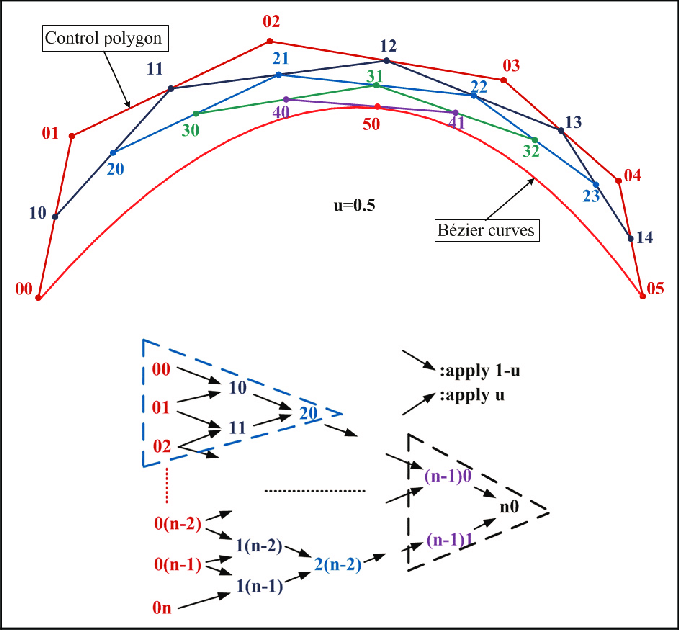
\includegraphics[height=9cm]{figures/General-process-of-De-Casteljau-algorithm.png}
    \caption{De-Casteljau Algorithm, from \cite{Wang-spline}}  
    \label{fig:De-casteljau-algo}
\end{figure}

\subsection{Derivative of Bezier curve}
\label{subsec:Derivative of Bezier curve}
\subsubsection{1st Method}
We use : 
\[
    p^{(k)} = \frac{ n!  }{ \left( n-k\right) ! } \sum_{k=0}^{n-k} \Delta^k P_i B _{ i }^{
    n-k} (t) 
\]
then we calculate $ \Delta ^k P_i  $ given by the De Casteljau algorithm on $ \Delta^kP_i
$.
When k = 0 
\[
\underbrace{
\begin{pmatrix*}
    P_0  \\
    P_1 \\
    \vdots \\
    P_n 
\end{pmatrix*}
\to  
\begin{pmatrix*}
    \Delta P_0  \\
    \Delta P_1 \\
    \vdots \\
    \Delta P_{n-1}  
\end{pmatrix*}
\to 
\begin{pmatrix*}
    \Delta^2 P_0  \\
    \Delta^2 P_1 \\
    \vdots \\ 
    \Delta^2 P_{n-2}  
\end{pmatrix*}}_{ \text{finite differences}} 
\underbrace{
\to 
P''(t) \frac{ 1 }{ n\left( n-1\right)  } }_{\text{De Casteljau}}
\]

\subsubsection{Second Method}
We do not need to calculate $ \Delta^k P_i  $. 
\begin{prop}[]
   \[
       P^{(k)} (t) = \frac{ n!  }{ \left( n-k\right) ! } \Delta ^k P _{ 0 }^{ \left( n-k\right)  } 
   \] 
    \label{def:}
\end{prop}

Thus, for $ k = 1 $ we have 
\[
    P'(t) = n\left( P _{ 1 }^{ (n-1)  } - P _{ 0 }^{ (n-1) } \right) 
\]
k=2 

\[
    P''(t) = n(n-1)\left( P _{ 1 }^{ (n-2)  } -2P _{ 1 }^{ (n-2) } +  P _{ 0 }^{ (n-2) } \right) 
\]
Intuition of the proof : 
\begin{align*}
    \Delta P_0  &= P_1 - P_0  \\
    \Delta P_1  &= P_2 - P_1  \\
    \text{ Which Gives }& \\
     &= \left( 1-t\right) \left( P_1 - P_0 \right) + t\left( P_2 - P_1 \right)  \\ 
      &= \left( 1-t\right) P_1 + tP_2  \\ 
       &= - \left( \left( 1-t\right) P_0 + P_1\right)  \\ 
\end{align*}


\section{Tutorial 2: Bézier Curves and Bernstein polynomials}
\label{sec:Tutorial 2: Bézier Curves and Bernstein polynomials}
\subsubsection{Exercise 1 (Bernstein polynomials)} 
Show the following : 
\begin{enumerate}
    \item Linear precision : 
        \[
            \sum_{i=0}^{n} \frac{ i }{ n  } B^n_i(t) = t \quad \forall t\in [0,1], \
            \forall n > 0, \ \forall i \in \set{ 0,\dots, n } 
        \]
    \item Recursive formula 
        \[
            B^n_i(t) = \left( 1-t\right) B _{ i }^{ n-1 } (t) + tB _{ i-1 }^{ n-1 } (t)
            \quad \forall n > 0, \ \forall i \in \set{ 0, \dots, n } 
        \]
    \item The family of Bézier polynomials $ \left( B_9\right) _{ 0\leq i \leq n  }^{  }
        $ is a basis of the space of polynomials of degree $ \leq n  $. 
\end{enumerate}
\subsubsection{Exercise 2}
Let $ P_0 $ and $ P_1 $ be two points of $ \mathbb{R}^d $. Descrie the Bézier curve
associated to $ P_0 $ and $ P_1 $. 

\subsubsection{Exercise 3}
Let $ \mathcal{ A }  $ be the affine space identified to $ \mathbb{R}^2 $ and $ \gamma $
be the parameterized curve 
\begin{align*}
    \gamma :  [0,1] &\to \mathbb{R}^2  \\ 
     t &\to \left( t,t^2\right)  \\ 
\end{align*}
\begin{enumerate}
    \item Express $ \gamma $ in the monomial basis. 
    \item Express $ \gamma $ in the Bernstein polyonimals basis. 
    \item Give the control polygon of $ \gamma $. Make a drawing with the curve and
        control polygon. 
\end{enumerate}

\subsubsection{Exercise 4}
Let $ [)_0, \cdots, P_6]  $ be a control polygon and : 
\begin{itemize}
  \item Express the condition on the $ P_i $ to ensure that the Bézier curve 
      \[
          P(t) = \sum_{i=0}^{6} P_iB^6_i(t) 
      \]
      is closed of class $ \mathscr{ C } ^2 $.
  \item Draw an example of such a control polygon.
\end{itemize}

\subsubsection{Exercise 5 (Bézier Function) }
A Bézier function is a curve of the form 
\begin{align*}
    f : [0,1] &\to \mathbb{R}\\
    t &\to \sum_{i=0}^{n} \lambda_i B_i^n(t) 
\end{align*}
Show that the graph  $ G(f) \coloneqq \set{ \left( x,f(x)\right) , x \in [0,1] }  $ of the
function $ f $ is a Bézier curve associated to the points $ P_i = \left( i/n, \lambda_i
\right)  $.

\subsubsection{Exercise 6}
Let $ f(t) = \sum_{i=0}^{n} \lambda_iB^n_i(t)  $ be a Bézier function. 
\begin{enumerate}
    \item Show that 
        \[
        \int\limits_{0}^{1} f(t) \ dt = \frac{ \lambda_0 + \dots + \lambda_n }{ n+1 } 
        \]
        hint : consider the primitive F of f
    \item In particular, show that 
        \[
            \int\limits_{0}^{1} B^n_i(t) = \frac{ 1 }{ n+1 } 
        \]
\end{enumerate}
\subsubsection{Exercise 7 (Degree elevation) }
The idea is to use the observation that a polynomial curve $ P $ of degree $ \leq n  $ can
be seen as a polynomial curve of degree $ \leq n+1 $, namely 
\[
    P(t) = \sum_{i=0}^{n} P_iB^n_i(t) = \sum_{i=0}^{n+1} Q_iB _{ i }^{ n+1 } (t) 
\] 
\begin{enumerate}
    \item Show that 
        \[
            B _{ i }^{ n  } (t) = \frac{ n+1 - i }{ n+1 } B _{ i }^{ n+1 } (t) + \frac{
            n+1  }{ i+1 } (t) 
        \]
    \item Calculate $ Q_i $ in terms of the $ P_j $'s
\end{enumerate}


\subsection{Solutions}
\label{subsec:Solutions}
\subsubsection{1) }
\begin{enumerate}
    \item 
        The first index vanishes, so we can rewrite the sum as 
        \[
            \sum_{i=1}^{n} \frac{ i }{ n  }  B _{ i  }^{ n  } (t) 
        \]
        Furthermore, 
        \[
        i \begin{pmatrix*}
            n   \\
            i  
        \end{pmatrix*}
        = \frac{ n\left( n-1\right) !  }{ \left( i-1\right) !\left( n-i\right) ! } = 
        n\begin{pmatrix*}
            n-1  \\
            i-1  
        \end{pmatrix*}
         
        \]
        Thus, we have, for the first iteration of the sum 
        \[
            \frac{ n   }{ n  } \frac{ \left( n-1\right) ! }{ \left( n-1\right) ! }  
            t\left( 1-t\right) ^{n-1} = t\left( 1-t\right) ^{n-1} = t \left( B _{ 0 }^{
            n-1 } (t) \right) 
        \]
        which allows us to rewrite the sum as 
        \[
            t\sum_{i=0}^{n} B _{ i }^{ n  } (t)  = t\left( 1\right) = t
        \]
    \item 
        \begin{align*}
            B _{ i }^{ n  } (t) &= \left( 1-t\right) B _{ i }^{ n-1 } (t) + tB _{ i-1 }^{
            n-1 } (t) \\
                                &= \left( 1-t\right) \begin{pmatrix*}
                                    n-1  \\
                                     i 
                                \end{pmatrix*}
                                t^i\left( 1-t\right)^{n-1-i} + t 
                                \begin{pmatrix*}
                                    n-1  \\
                                    i-1  
                                \end{pmatrix*}
                                t^{i-1}\left( 1-t\right) ^{n-1 - (i-1)}\\ 
                                 &= \begin{pmatrix*}
                                     n-1  \\
                                     i  
                                 \end{pmatrix*}
                                 t^i\left( 1-t\right) ^{n-i} +
                                 \begin{pmatrix*}
                                     n-1  \\
                                     i-1  
                                 \end{pmatrix*}
                                 t^i\left( 1-t\right) ^{n-i}\\
                                  &= \left( \begin{pmatrix*}
                                      n-1  \\
                                      i  
                                  \end{pmatrix*}
                                  + 
                                  \begin{pmatrix*}
                                      n-1  \\
                                      i-1  
                                  \end{pmatrix*}
                              \right) t^i\left( 1-t\right) ^{n-i}  \\
                               &= \begin{pmatrix*}
                                   n   \\
                                   i  
                               \end{pmatrix*}
                               t^i\left( 1-t\right) ^{n-i} = B _{ i }^{ n  } (t) \\ 
            \end{align*}
        \item To show $ B _{ i }^{ n  } (t) $ as a basis of the space of polynomials of
            degree $ \leq n  $ we use derivation. 
            Consider how 
            \[
                B _{ i }^{ n  } (t) \implies \begin{pmatrix*}
                    n   \\
                    i  
                \end{pmatrix*} t^i
                \left( P \right)  
            \]
            where $ P $ is some polynomial. Then we can write this as a sum under the form 
            \[
            \alpha_0\left( P\right) + \alpha_1t\left( P\right) + \cdots  + \alpha_nt^n = 0
            \]
            We check each $ \alpha_i $. Firstly, taking the derivative of this polynomial
            gives us 
            \[
                \alpha_1\left( P\right) + \cdots  + n\alpha_nt^{n-1} = 0
            \]
            Then $ \alpha_0 = 0 $, this can be done iteratively for each $ \alpha_i $.
            Then $ B _{ i  }^{ n  } (t)  $ is a linear independent set and a basis for
            polynomials of degree $ \leq n $.  
\end{enumerate}

\subsubsection{2)}
The Bézier curve consisting of only 2 points is the straight line :  
\begin{align*}
    P(t) &= \sum_{i=0}^{1} P_iB _{ i }^{ n  } (t) \\
     &= P_0\left( 1-t\right) + P_1t \\ 
      &= P_0 + \left( P_1 - P_0\right) t \\ 
\end{align*}

\subsubsection{3)}
\begin{enumerate}
  \item The monomial basis has representation 
      \[
      \begin{pmatrix*}
          1  \\
          0  
      \end{pmatrix*}
      t + \begin{pmatrix*}
          0  \\
          1  
      \end{pmatrix*}
      t^2
      \]
  \item Bernstein basis is given by : 
      \[
          B _{ 0 }^{ 2 } (t) = \left( 1-t\right)^2; \quad B _{ 1 }^{ 2 } (t) = 2t\left( 1-t\right)
           ; \quad B _{ 2 }^{ 2 } (t) = t^2
      \]
      which results in the following : 
     \[
     \begin{pmatrix*}
         0  \\
         0  
     \end{pmatrix*}
     B _{ 0 }^{ 2 } (t) + 
     \begin{pmatrix*}
         \frac{ 1 }{ 2 }   \\
         0 
     \end{pmatrix*}
     B _{ 1 }^{ 2 } (t) + \begin{pmatrix*}
         1  \\
         1  
     \end{pmatrix*}
     B _{ 2 }^{ 2 } (t)
     \]
 \item The curve is given by :  
\begin{figure}[ht]
    \centering
    \incfig{e4p3}
    \caption{e4p3}
    \label{fig:e4p3}
\end{figure}
\end{enumerate}

\subsubsection{4)}
\begin{itemize}
  \item In order to ensure that the Bézier curve 
      \[
          P(t) = \sum_{i=0}^{6} P_iB _{ i }^{ 6 } (t) 
      \]
      to be closed of class $ \mathscr{ C } ^2 $ we must have 
      \begin{enumerate}
          \item $P(0) = P(1)$ 
          \item $ P'(0) = P'(1) $
          \item $ P''(0) = P''(1) $
      \end{enumerate}
      Thus, 
      \begin{enumerate}
          \item \[ P_0 = P_n \]
          \item 
              \begin{align*}
                  P'(0) = 6\left( P_1 - P_0\right) &= P'(1) = 6\left( P_5 - P_6\right) \\
                  \vv{P_1P_0} &= \vv{P_5P_6} 
              \end{align*}
          \item 
              \begin{align*}
                  P''(0) = 30\left( P_2 - 2P_1 + P_0\right) &= P''(1) = 30\left( P_4 - 2P_5
                  + P_6\right) \\
                   &\text{ since } P_0 = P_6 \\ 
                  P_2 - 2P_1 &= P_4 - 2P_5 \\
                  \vv{P_2P_4} &= 2\vv{P_1P_5} \\ 
              \end{align*}
      \end{enumerate}
        This system of equations results in the figure : 
\begin{figure}[ht]
    \centering
    \incfig{t2e4}
    \caption{Closed of Class $ \mathscr{ C } ^2 $}
    \label{fig:t2e4}
\end{figure}
\end{itemize}

\subsubsection{5)}
This is found through simple computation. We take 
\[
P_i = \begin{pmatrix*}
    \frac{ i }{ n  }   \\
    \lambda_i   
\end{pmatrix*}
\]
Then 
\begin{align*}
    \sum_{i=0}^{n } \begin{pmatrix*}
        i/n   \\
        \lambda_i   
    \end{pmatrix*}
    B _{ i  }^{ n  } (t) &= \begin{pmatrix*}
        \sum_{i=0}^{n } \frac{ i }{ n  } B _{ i  }^{ n  } (t)   \\
        \sum_{i=0}^{n } \lambda_i B _{ i  }^{ n  } (t)   
    \end{pmatrix*} \\ 
     &= \begin{pmatrix*}
         t  \\
         f(t)  
     \end{pmatrix*}
      \\ 
\end{align*}

\subsubsection{6)}
\begin{enumerate}
    \item 
    \begin{align*}
        \int\limits_{0}^{1} f(t) \ dt
    \end{align*}
\item 
\end{enumerate}

\subsubsection{7)}
\begin{enumerate}
    \item 
        \begin{align*}
            &\frac{ n+1-i }{ n+1 } B _{ i }^{ n+1 } (t) + \frac{ i+1 }{ n+1 }B _{ i+1 }^{
        n+1 } (t)  \\ 
            &=  \frac{ n+1-i }{ n+1 } \begin{pmatrix*}
                n+1  \\
                i  
            \end{pmatrix*}
            t^i\left( 1-t\right) ^{n+1-i} + \frac{ i+1 }{ n+1 } \begin{pmatrix*}
                n+1  \\
                i+1  
            \end{pmatrix*}
            t^{i+1}\left( 1-t\right) ^{n+1-(i+1)} \\ 
            &=  
                \frac{ n! }{ i!\left( n-i\right) ! } 
            t^i\left( 1-t\right) ^{n+1-i} + 
            \frac{n! }{ i!\left( n - i\right)!} 
            t^{i+1}\left( 1-t\right) ^{n-i} \\ 
             &= \begin{pmatrix*}
                 n   \\
                 i  
             \end{pmatrix*}
             t^i\left( 1-t\right) ^{n-i} \left( \left( 1-t\right) + t\right)    
             \\
             &= B _{ i  }^{ n  } (t) \\  
               \\ 
        \end{align*} 
    \item We begin by expanding using the form above : 
        \begin{align*}
            \sum_{i=0}^{n } P_iB _{ i }^{ n  } (t) &= \sum_{i=0}^{n }P_i \left( \frac{ n+1-i
            }{ n+1 }B _{ i }^{ n+1 } (t) + \frac{ i+1 }{ n+1 } B _{ i+1 }^{ n+1 }
        (t)\right) \\
                                                   &= \sum_{i=0}^{n} \frac{ n+1-i }{ n+1 }
                                                   P_iB _{ i }^{ n+1 } (t) +
                                                   \sum_{i=1}^{n+1} \frac{ i }{ n+1 } 
                                                   P_{i-1}B _{ i }^{ n+1 }  \\ 
                                                   &= P_0B _{ 0 }^{ n+1 } (t) +
                                                   \sum_{i=1}^{n} \left( P_i \frac{ n+1-i
                                                   }{ n+1 } + P_{i-1} \frac{ i }{ n+1 }
                                               \right) B _{ i }^{ n+1 } (t) + P_nB _{ n+1
                                           }^{ n+1 }  \\ 
        \end{align*} 
\end{enumerate}



\chapter{Curves in the Plane}
\section{Introduction}
\label{sec:Introduction}

To represent them, we use 
\begin{defn}[Parametrized Curves]
    \begin{align*}
        \gamma : [a,b] &\to \mathbb{R}^d \\
        t &\to \gamma(t)  
    \end{align*}
    \label{def:Parametrized Curves}
\end{defn}

\begin{figure}[ht]
    \centering
    \incfig{planar-curve}
    \caption{Parametrized Planar Curve}
    \label{fig:planar-curve}
\end{figure}


\begin{defn}[Implicit Curves]
    Let $ f : \mathbb{R}^2 \to \mathbb{R} $
    then $ f^{-1} ( \set{ 0 } ) = \set{ (x,y) \in \mathbb{R}^2, f(x,y) = 0 }  $
    is a curve.
    \label{def:Implicit Curves}
\end{defn}

\begin{exmp}[]
    \[
        f(x,y) = x^2 + y^2 -1 
    \]
\end{exmp}

\begin{figure}[ht]
    \centering
    \incfig{example313}
    \caption{Example 3.1.3}
    \label{fig:example313}
\end{figure}


\begin{defn}[Graphs of Functions]
    $ \varphi : [a,b] \to \mathbb{R} $. 
    \[
        \text{graph} \left( \varphi\right) = \set{ \left( t, f(t) \right) , t \in [a,b]  } 
    \]
    \label{def:Graphs of Functions}
\end{defn}

\newpage
\begin{exmp}[]
    $ \varphi = \sqrt{1 - t^2}  $ and $ t \in [-1,1]  $ then 
\end{exmp}

\begin{figure}[ht]
    \centering
    \incfig{example315}
    \caption{Example 3.1.5}
    \label{fig:example315}
\end{figure}





\section{Generalities on Paramaterized Curves}
\label{sec:Generalities on Paramaterized Curves}
\subsection{Reminder}
\label{subsec:Reminder}
Let $ f:[a,b] \to \mathbb{R}^2\in \mathscr{ C } ^n $ and $ t_0 \in [a,b] $ then 
\[
    f(t) = f(t_0) + \left( t-t_0\right) f'(t_0) + \frac{ \left( t-t_0\right) ^2 }{ 2!  }
    f''(t_0) + \dots + \frac{ \left( t-t_0\right) ^n }{ n! } f^{(n)} (t_0) + \mathcal{ O
    } \left( \left( t-t_0\right) ^n\right) 
\]

In particular, 
\[
    \frac{ f(t) - f(t_0)  }{ t - t_0  } = f'(t_0) 
\]
let curve be $ \mathscr{ C } = \set{ f(t) }  $ and $ f(t_0) \in \mathscr{ C }  $ and $
f'(t_0)  $ is a vector tangent to $ \mathscr{ C }  $ at $ f(t_0)  $. 

Some notes about 2nd derivative and how it "attracts" the curve. 


\[
    f(t) = f(t_0) + f^{(p)}(t_0) \frac{ \left( t-t_0\right) ^p }{ p! } + \dots + 
    f^{(q)}(t_0) \frac{ \left( t-t_0\right) ^q }{ q! } + \mathcal{ O  } \left( \dots\right) 
\]
p is the smallest k such that $ f^{(k)}(t_0) \neq 0 $ and q is smallest q such that 
\[
    \left( f^{(q)}(t_0),f^{(k)}(t_0)\right)   \text{ independent } 
\]
\newpage
\begin{figure}[ht]
    \centering
    \incfig{linearinependenceoftan}
    \caption{linear independence between derivatives}
    \label{fig:linearinependenceoftan}
\end{figure}

Certain characteristics of the curve can be given by the values of $ p,q $. 


\begin{figure}[ht]
    \centering
    \incfig{pqcurvecharacteristics}
    \caption{pqCurveCharacteristics}
    \label{fig:pqcurvecharacteristics}
\end{figure}

These values then blah blah blah
$ \\ $
\newpage


\section{Parametrization and Geometric Curves}
\label{sec:Parametrization and Geometric Curves}
\begin{defn}[Parametrized Curve]
    A Paramterized curve of class $ \mathscr{ C } ^k $ is a map $ f: I \subset
    \mathbb{R}\to \mathbb{R}^3 \in \mathscr{ C } ^k$, where I is a union of intervals. We
    denote $ \left( I, f\right)  $ such a curve.
    \label{def:Parametrized Curve}
\end{defn }

Remark : 
\[
    F(I) \coloneqq \mathscr{ C } 
\]
is the geometric support. Interval connected $ \implies \mathscr{ C }  $ is connected. 
I compact set $ \implies \mathscr{ C }  $ compact set. 
$ \\ $
Remark : 
$ \\ $
Some curve may have 2 paramterization without the same regularity. 
\begin{exmp}[]
    \begin{align*}
        t &\to \left( t, t^{3/2}\right) t > 0  \\ 
        t &\to \left( \left | t \right | , - \sqrt{t^3}\right) t \leq 0  \\ 
    \end{align*}
    another parametrization is 
    \[
        t \to \left( t^2, t^3\right) \in \mathscr{ C } ^{\infty} 
    \]
\end{exmp}
 

\newpage 
\subsection{ReParametrization}
\label{subsec:ReParametrization}
Let $ f : I \to \mathbb{R}^3 $ param curve in $ \mathscr{ C } ^k $ and $ e : J \to I $ is
a $ \mathscr{ C } ^k $ diffeomorphism (bijective, $ e'(x) \neq 0, \mathscr{ C } ^k $. 
Then $ f \circ e : J \to \mathbb{R}^3 $ has the same "geometric curve" and we say that 
\begin{itemize}
  \item $ f\circ e $ is a reparametrization of $ f $
  \item $ e $ is called an admissible change of variable
\end{itemize}


\begin{figure}[ht]
    \centering
    \incfig{reparamaterized-curve}
    \caption{Reparamaterized Curve}
    \label{fig:reparamaterized-curve}
\end{figure}


We consider the following equivalence class 
\begin{defn}[Equivalence Class for Curves]
    $ \\ $
    $ \left( I,f\right) \sim \left( J,g\right)  $ if 
    $
    \exists e : J \to I,  g = f \circ e  \text{ e admissible change of variable} 
    $
    \label{def:}
\end{defn}

\begin{defn}[Geometric Curve]
    A geometric curve is an equivalence class of this relation
    \label{def:Geometric Curve}
\end{defn}

\section{Regular Curve}
\label{sec:Regular Curve}

\begin{defn}[Regular Curve]
    Let $ k \geq 1 $. 
    We say that a paramatrized curve $ \left( f,I\right)  $ of class $ \mathscr{ C } ^k $
    is regular if 
    \[
        f'(t) \neq 0 \ \forall t \in I
    \]
    A geometric curve is regular if there exists a paramatrized which is regular. 
    \label{def:Regular Curve}
\end{defn}

If $ \mathscr{ C } $ is of class $ \mathscr{ C } ^1 $, then there exists $ f: I \to
\mathscr{ C }  $, where $ \mathscr{ C } = f\left( I\right)  $ 
\[
    f'(t) \neq 0 \quad f'(t) \text{ is tangent to } \mathscr{ C } ^k \text{ at } f(t)
\]

If $ \left( I,f\right)  $ is regular then every reparametrization $ \left( J,g \right)  $ 
is also regular. Indeed : $ \forall t, \ f'(t) \neq 0  $ gives 
\[
    g = f \circ e \implies \forall t,  \ g'(t) = \underbrace{f'(e(t))}_{\neq 0} \times 
    \underbrace{e'(t)}_{\neq 0}  \neq 0
\]

\begin{exmp}[]
    A line segment in $ \mathbb{R}^2 $ with $ t \to \left( t, at+b\right)  $ regular,
    can also be
    reparametrizated by $ t\to \left( t^3, at^3+b\right)  $ non regular. The reason for this is 
    \[
        f'(t) = \left( 3t^2, 3at^2\right) = 0 \text{ at } x = 0
    \]
\end{exmp}
\subsubsection{Remark}
This curve does not admit a regular paramatrization. 

    
\begin{figure}[ht]
    \centering
    \incfig{regular-and-non-regular-curves}
    \caption{Regular and Non-regular curves}
    \label{fig:regular-and-non-regular-curves}
\end{figure}

However, this is not to say that there does not exist parametrizations of these figures,
it is just to say that $ f'(a) = 0 $ where a is the non-smooth point. 

Furthermore, we have 


\begin{figure}[ht]
    \centering
    \incfig{c1-but-not-c2}
    \caption{ $ \mathscr{ C } ^1 $ but not $ \mathscr{ C } ^2 $}
    \label{fig:c1-but-not-c2}
\end{figure}

This curve is $ \mathscr{ C } ^1 $ since $ f''(x) = 0 $. 
\newpage 

\section{Metric Properties of Curves}
\label{sec:Metric Properties of Curves}
\subsection{Length of curves}
\label{subsec:Length of curves}
\begin{defn}[Length of a curve]
    Let $ f : I = [a,b] \to \mathbb{R}^d $. We see that the straight line segments 
    obviously have less length than $ \mathscr{ C }  $. $ \\ $
    Let $ \mathscr{ S }  = \set{ \text{ subdivisions } a=t_0 < \dots < t_n = b } $.

    For $ s \in \mathscr{ S }   $ we denote 
    \[
        \gamma(s) = \sum_{i=0}^{N-1} \| f(t_{i+1}) - f(t_i) \|^{ }_{ }  
    \]If $ \set{ \gamma(s), s \in \mathscr{ S }   }  $ is bounded we say that $ f $ is
    rectifiable. Its lengh is defined by 
    \[
        \gamma(f) = \sup_{s \in \mathscr{ S } } \gamma(s)
    \]
    Then If $ f:[a,b] \to \mathbb{R}^d $ is $ \mathscr{ C } ^1 $ then $ f $ is rectifiable
    and 
    \[
        \gamma(f) = \int\limits_{a}^{b} \| f'(t) \|^{ }_{ } \ dt
    \]
    \label{def:Length of a curve}
\end{defn}
Sketch of proof $ \\ $

\begin{align*}
    \int\limits_{a}^{b} \| f'(t)  \|^{ }_{ } \ dt &= \sum_{i=1}^{n-1}
    \int\limits_{t_i}^{t_{i+1}} \| f'(t)  \|^{ }_{ } \ dt \\ 
\end{align*}
The right hand side of this term gives us 
\begin{align*}
     &\sim \left( t_{i+1} - t_i \right) \| f'(t) \|^{ }_{ }   \\ 
     &\sim \left( t_{i+1} - t_i \right) \frac{ \| f(t_{i+1} - f(t_i)  )  \|^{ }_{ }  }{
     \left | t_{i+1} - t_i \right |  }   \\ 
\end{align*}

\begin{figure}[ht]
    \centering
    \incfig{length-of-a-curve}
    \caption{Length of a Curve}
    \label{fig:length-of-a-curve}
\end{figure}





\subsection{Arc Length Parametrization}
\label{subsec:Arc Length Parametrization}
\begin{defn}[]
    Let $ \left( I,f\right) \in \mathscr{ C } ^1 $ where $ I = [a,b] ,\ t_0 \in I $. We
    call arc-length the map 
    \begin{align*}
        \simga: I &\to \mathbb{R}  \\
        t &\to \int\limits_{t_0}^{t} \| f'(\mu) \|^{ }_{ } \ d\mu \\ 
    \end{align*} 
    \label{def:}
\end{defn}
\subsubsection{Remark}
$ \left | \sigma(t) \right |  $ is the length of the curve between $ f(t)  $ and $ f(t_0)
$ where $ \sigma(t) < 0 \iff t<t_0 $
\subsubsection{Remark}
If $ f $ is regular then $ \sigma  $ is strictly increasing and $ \sigma'(t) = \| f'(t)
\|^{ }_{ } > 0 $, therefore, $ \sigma  $ is an admissable change of variable of class $
\mathscr{ C } ^1 $

\begin{defn}[]
    $ f\circ \sigma^{-1} $ is an arc-length paramatrization of the curve. 
    \label{def:}
\end{defn}
So every $ \mathscr{ C } ^1 $ regular curve admits an arc-length paramatrization.
We use, by convention, $ S $ as the parameter of the arc-length parametrization.

\begin{figure}[ht]
    \centering
    \incfig{arc-length-paramatrization}
    \caption{Arc-length Paramatrization}
    \label{fig:arc-length-paramatrization}
\end{figure}








\begin{prop}[]
    \begin{itemize}
      \item  The arc-length paramatrization is unique up to the parameter $ t_0 $ if $ I = [a,b],\
    t_0 = a $.
\item $ \forall s \in J, \ \| f'(s) \|^{ }_{ } = 1 $ if $ f $ arc-length param 
\item $ \forall s \in J, f'(s) \perp f''(s)  $ for $ f $ arc-length
    \end{itemize}  
\end{prop}
\begin{proof}
    Let $ g $ be any parametrization and $ f = g \circ \sigma^{-1}  $. Then 
    \[
        \forall s \ f'(s) = g'\left( \sigma^{-1} (s) \right) \times \left(
        \sigma^{-1}\right) '(s) = \frac{ g'\left( \sigma^{-1}(s)\right)  }{ \| g'\left(
    \sigma^{-1}(s)\right)  \|^{ }_{ }  } 
    \]
    where 
    \[ \left( \sigma^{-1}\right)' (s) = \frac{ 1 }{ \sigma'\left(\sigma^{-1}(s)\right) } = 
    \frac{ 1 }{ \| g'\left( \sigma^{-1}(s)\right)  \|^{ }_{ }  } \]
    Then $ \| f'(s) \|^{ }_{ } = 1 $ and 
    \[
        \forall s \in J \ \| f'(s) \|^{ 2}_{ } = \langle f'(s) , f'(s) \rangle = 1
    \]
    We derive, $ \forall s \in J  $
    \[
        2 \langle f''(s)  , f'(s)  \rangle = 0 \implies f''(s) \perp f'(s)
    \]
\end{proof}

\section{Planar Curves}
\label{sec:Planar Curves}
\subsection{Serret-Fresnet Frame}
\label{subsec:Serret-Fresnet Frame}
Let $ f : I \to \mathbb{R}^2, \in \mathscr{ C } ^1 $-regular. Then 
\[
    T(t) = \frac{ f'(t)  }{ \| f'(t) \|^{ }_{ }  } \quad N(t) = \text{rot}_{ \frac{ \pi }{
    2}} \left( T(t)\right) 
\]
So $ \left( f(t), \boldsymbol{T}(t), \boldsymbol{N} (t) \right)  $ is a frame that is
called the Serret-Fresnet Frame.

\subsubsection{Remark}
If arc-length then we have 
\[
    T(s) = f'(s) \qquad N(s) = \text{rot} _{ \frac{ \pi }{ 2 } }\left( T(s)\right) 
\]

\subsection{Curvature}
\label{subsec:Curvature}
\begin{defn}[Curvature]
    Let $ f : I \to \mathbb{R}^2 $ arc-length. The curvature at $ f(s)  $ is defined by 
    \[
        k(s) \coloneqq \langle f''(s)  , N(s)  \rangle = \pm \| f''(s) \|^{ }_{ } 
    \]
    \label{def:Curvature}
\end{defn}
\begin{prop}[]
    Let $ f : I \to \mathbb{R} $ any parametrization. Then 
    \[
        k(u) = \frac{ \text{det} \left( f'(u), f''(u) \right)  }{ \| f'(u) \|^{3 }_{ }  } 
    \]
    \label{def:}
\end{prop}

\begin{proof}
    We denote $ \overline{f} = f \circ \sigma^{-1}  $ the arc-length parametrization. We
    put $ u = \sigma^{-1}(s)  $. Then 
    \begin{align*}
        \overline{f}'(s) &= f'\left( \sigma^{-1}(s) \right) \frac{ 1 }{ \| f'\left( \sigma^{-1}
        (s)\right)  \|^{ }_{ }  }  \\
                     &= \frac{ f'(u) }{ \| f'(u) \|^{ }_{ }  }  \\ 
    \end{align*}
    We derive again 
    \begin{align*}
        \overline{f}''(s)  &= \frac{ f''(u) }{ \| f'(u) \|^{2 }_{ }  } + f'(u) \frac{ d }{
        ds}  \\ 
    \end{align*}
    where $ \frac{ d }{ ds }  $ is the real value result of the rhs above 
    \begin{align*}
        \text{det} \left( \overline{f}'(s), \overline{f}''(s) \right)  &= \text{det}
        \left( \frac{ f'(u) }{ \| f'(u) \|^{ }_{ }} , \frac{ f''(u) }{ \| f'(u) \|^{2 }_{
            }}
        + \lambda u f'(u)   \right)  \\ 
                                                                       &=
                                                                       \frac{\text{det}
                                                                       \left(f'(u), f''(u)
                                                                   \right)  }{ \| f'(u)
                                                               \|^{3 }_{ }   }  \\ 
    \end{align*}
    And 
    \begin{align*}
        \text{det} \left( \overline{f}'(s) , \overline{f}''(s) \right) &= \text{det} \left( T(s),
        k(s)N(s)\right) \\
        &= k(s)
    \end{align*}
    since, 
    \[
        f''(s) = k(s)N(s) 
    \]
    \[
        k(s) \coloneqq \langle f''(s) , N(s) \rangle = \pm \| f''(s) \|^{ }_{ } 
    \]
\end{proof}

\begin{figure}[ht]
    \centering
    \incfig{curvature}
    \caption{curvature}
    \label{fig:curvature}
\end{figure}








\subsection{Osculating Circle and Center of Curvature}
\label{subsec:Osculating Circle and Center of Curvature}
\begin{defn}[]
    \[
        c(t) = f(t) + \frac{ 1 }{ k(t) } N(t) 
    \]
    is called the center of curvature. 
    \[
        \frac{ 1 }{ \left | k(t) \right |  } 
    \]
    is the radius of curvature at $ f(t) $
    The circle 
    \[
        \mathscr{ C } \left( c(t), \frac{ 1 }{ \left | k(t) \right |  } \right) 
    \]
    The evolute of $ f $ is the set of centers of curvatures.
\end{defn}


\subsection{Serret-Fresnet Formula}
\label{subsec:Serret-Fresnet Formula}
\begin{prop}[]
    \[
        T'(s) = k(s)N(s) \qquad N'(s) = -k(s)T(s)  
    \]
    lhs done is done, and rhs is by definition 
\end{prop}

\subsection{Total Curvature}
\label{subsec:Total Curvature}

\begin{ftheo}[Total Curvature]
    Let $ f: I \subset \mathbb{R}\to \mathbb{R}^2 $ planar curve parametrized by
    arc-length, then 
    \[
        \int\limits_{a}^{b} k(s) \ ds = \theta(a,b)
    \]
    is the angle between the two tangents at a and b.
    \label{th:Total Curvature}
\end{ftheo}


\begin{proof}
    \[
        f(s) = \begin{pmatrix*}
            x(s)  \\
            y(s)  
        \end{pmatrix*}
        \quad \theta (s) = \left( (o,x) , T(s) \right) 
    \]
    where $ o  $ is the angle between tangent and the x? 
    Then 
    \[
        T(s) = \begin{pmatrix*}
            \cos \theta (s)   \\
            \sin \theta (s)   \\
        \end{pmatrix*}
        \quad 
        N(s) = 
        \begin{pmatrix*}
            -\sin \theta (s)  \\
            \cos \theta (s)   
        \end{pmatrix*}
        
    \]
    However, 
    \[
        T'(s) = k(s) N(s) \quad \text{ and } T'(s) = \theta '(s) N(s) 
    \]
    then 
    $ \theta '(s) = k(s)  $. 
    then 
    \[
        \int\limits_{a}^{b} \theta '(s) ds = \theta(b) - \theta(a) 
    \]
    which is the difference between the angles. 
\end{proof}

\begin{figure}[ht]
    \centering
    \incfig{total-curvature}
    \caption{Total Curvature}
    \label{fig:total-curvature}
\end{figure}

In figure \ref{fig:total-curvature} we have $ \theta_1\left( a,b\right) = \theta_2\left(
a,b\right) = \theta_3\left( a,b\right) + 6\pi $. We defined the "winding number" as an
index refering to the full revolutions around the a curve that is closed of class $
\mathscr{ C } ^2 $.  

\[
    k = \frac{ l }{ 2\pi  } \int\limits_{a}^{b} k(s) \ ds \in \mathbb{Z}
\]


\begin{figure}[ht]
    \centering
    \incfig{winding-numbers}
    \caption{Winding Numbers}
    \label{fig:winding-numbers}
\end{figure}

\subsubsection{Concluding Thoughts}
\begin{itemize}
  \item Metrics of a curve are given by the 1st derivative
  \item Them shape of a curve is given by the second derivative. 
  \item Arc length parametrization gives constant speed along the curve 
\end{itemize}







%\chapter{The Time Variable}
\section{Class notes} 
\includepdf[pages={29-34}]{sources/polyEDP-M1-main.pdf}

%\chapter{The Transport Equation}
\section{Class notes} 
\includepdf[pages={35-40}]{sources/polyEDP-M1-main.pdf}

%\chapter{The Wave Equation}
\section{Class notes} 
\includepdf[pages={41-46}]{sources/polyEDP-M1-main.pdf}

%\chapter{The Diffusion Equation}
\section{Class notes} 
\includepdf[pages={47-52}]{sources/polyEDP-M1-main.pdf}

%\appendix 
\chapter{Class notes} 
\includepdf[pages={53-61}]{sources/polyEDP-M1-main.pdf}

\chapter{Ordinary Differential Equations} 
\section{Elementary Integration Methods}
\label{sec:Elementary Integration Methods}
\subsection{First Order Equations}
\label{subsec:First Order Equations}
\subsubsection{Seperable Variables}
Consider
\begin{equation}
    y '= f(x) g(y)      
    \label{eq:seperable}
\end{equation}
can be serperated and divided such that 
\[
\int\limits_{ }^{ } \frac{ dy }{ g(y)  } = \int\limits_{ }^{ } f(x) \ dx + C
\]
A special case of this is $ y'= f(x) y $, which has solution 
\[
    y(x) = CR(x) , \qquad R(x) = exp\left( \int\limits_{ }^{ } f(x) \ dx\right) 
\]

\subsubsection{Inhomogeneous Linear Equation}
\begin{equation}
    y ' =  f(x) y + g(x) 
    \label{eq:inhomoLineq}
\end{equation}
Then the solution is given by 
\[
    y = e _{  }^{ - \int\limits_{ }^{ } f(x)\  dx    } \left( C + \int\limits_{ }^{ } g(x)
    e _{  }^{ \int\limits_{ }^{ } f(x) \ dx } \ dx\right)  
\]


\subsection{Linear Differential Equations}
\label{subsec:Linear Differential Equations}
\subsubsection{Equations with Constant Coefficients}
\begin{equation}
    y _{  }^{ (n) } (x) = 0
    \label{eq:constCoefHomo}
\end{equation}
Integrating n times gives 
\[
    y(x) = C_1x^{n-1} +C_2x^{n-2} + \cdots + C_{n}  
\]
The general equation with constant coefficients is  
\[
    y _{  }^{ (n)  } + A_{n-1}y _{  }^{ (n-1) } + \dots + A_0y = 0
\]



\printbibliography

\end{document}
